
% options:
% thesis=B bachelor's thesis
% thesis=M master's thesis
% czech thesis in Czech language
% english thesis in English language
% hidelinks remove colour boxes around hyperlinks

\documentclass[thesis=M,english]{FITthesis}[2012/10/20]

% \usepackage[utf8]{inputenc} % LaTeX source encoded as UTF-8
% \usepackage[latin2]{inputenc} % LaTeX source encoded as ISO-8859-2
% \usepackage[cp1250]{inputenc} % LaTeX source encoded as Windows-1250

\usepackage{graphicx} %graphics files inclusion
%\usepackage{subfig}
\usepackage{amsmath}
\usepackage{amssymb}
\usepackage[chapter]{algorithm} % http://ctan.org/pkg/algorithms
\usepackage[noend]{algpseudocode} % http://ctan.org/pkg/algorithmicx
\usepackage{pseudocode}
\usepackage{comment}
\usepackage{enumitem}
\usepackage{amssymb}
\usepackage{caption}
\usepackage{subcaption}
\usepackage[section]{placeins}

\usepackage[hang,flushmargin]{footmisc}


\usepackage{dirtree} %directory tree visualisation

% % list of acronyms
% \usepackage[acronym,nonumberlist,toc,numberedsection=autolabel]{glossaries}
% \iflanguage{czech}{\renewcommand*{\acronymname}{Seznam pou{\v z}it{\' y}ch zkratek}}{}
% \makeglossaries

%%%%%%%%%%%% own commands %%%%%%%%%%%%%%%%%%
\newcommand{\matr}[1]{\mathbf{#1}} 
\newcommand{\argmax}{\mathop{\mathrm{argmax}}}

\newcommand\footnoteref[1]{\protected@xdef\@thefnmark{\ref{#1}}\@footnotemark}

\makeatletter
\def\BState{\State\hskip-\ALG@thistlm}
\makeatother
%\newcommand{\max}{\mathop{\mathrm{max}}}

% % % % % % % % % % % % % % % % % % % % % % % % % % % % % % 
% EDIT THIS
% % % % % % % % % % % % % % % % % % % % % % % % % % % % % % 

\department{Department of Theoretical Computer Science }
\title{Learning Methods for Continuous-Time Hidden Markov Models}
\authorGN{Luk{\' a}{\v s}} %author's given name/names
\authorFN{Lopatovsk{\' y}} %author's surname
\author{Luk{\' a}{\v s} Lopatovsk{\' y}} %author's name without academic degrees
\authorWithDegrees{Bc. Luk{\' a}{\v s} Lopatovsk{\' y}} %author's name with academic degrees
\supervisor{Ing. Daniel Va{\v s}ata, Ph.D.}
\acknowledgements{THANKS (remove entirely in case you do not with to thank anyone)}
\abstractEN{Summarize the contents and contribution of your work in a few sentences in English language.}
\abstractCS{V n{\v e}kolika v{\v e}t{\' a}ch shr{\v n}te obsah a p{\v r}{\' i}nos t{\' e}to pr{\' a}ce v {\v c}esk{\' e}m jazyce.}
\placeForDeclarationOfAuthenticity{Prague}
\keywordsCS{Replace with comma-separated list of keywords in Czech.}
\keywordsEN{HMM, CT-HMM.}
\declarationOfAuthenticityOption{1} %select as appropriate, according to the desired license (integer 1-6)
% \website{http://site.example/thesis} %optional thesis URL


\begin{document}

% \newacronym{CVUT}{{\v C}VUT}{{\v C}esk{\' e} vysok{\' e} u{\v c}en{\' i} technick{\' e} v Praze}
% \newacronym{FIT}{FIT}{Fakulta informa{\v c}n{\' i}ch technologi{\' i}}

\setsecnumdepth{part}

\begin{introduction}
	This is the master thesis. welcome!
	bibtex test: \cite{Sk01}
	\section{Motivation and objectives}
	About a discrete model [inspired by Rabiner? ] and why it is not satisfactory  %(as http://delivery.acm.org/10.1145/350000/343402/p162-aziz.pdf?ip=147.32.98.33&id=343402&acc=ACTIVE%20SERVICE&key=D6C3EEB3AD96C931%2E9BD1EC80ACA8C1C5%2E4D4702B0C3E38B35%2E4D4702B0C3E38B35&CFID=702042173&CFTOKEN=62280276&__acm__=1481276923_1a71eb623e1c42d4c8e9b84178eb248f)	
	Add articles and DP that have done it before - less or more successfully 
	
The figure example \ref{fig:gb}.

CT-HMM is the natural extension of discrete-time model, that ..

%\section{Continuous-Time Hidden Markov Model}
[move or delete]When we mention continuous-time hidden Markov model, we will consider its finite states variant. Also the infinite states models exist, but they are out of the scope for these thesis.[]


\begin{figure}[h]
\centering
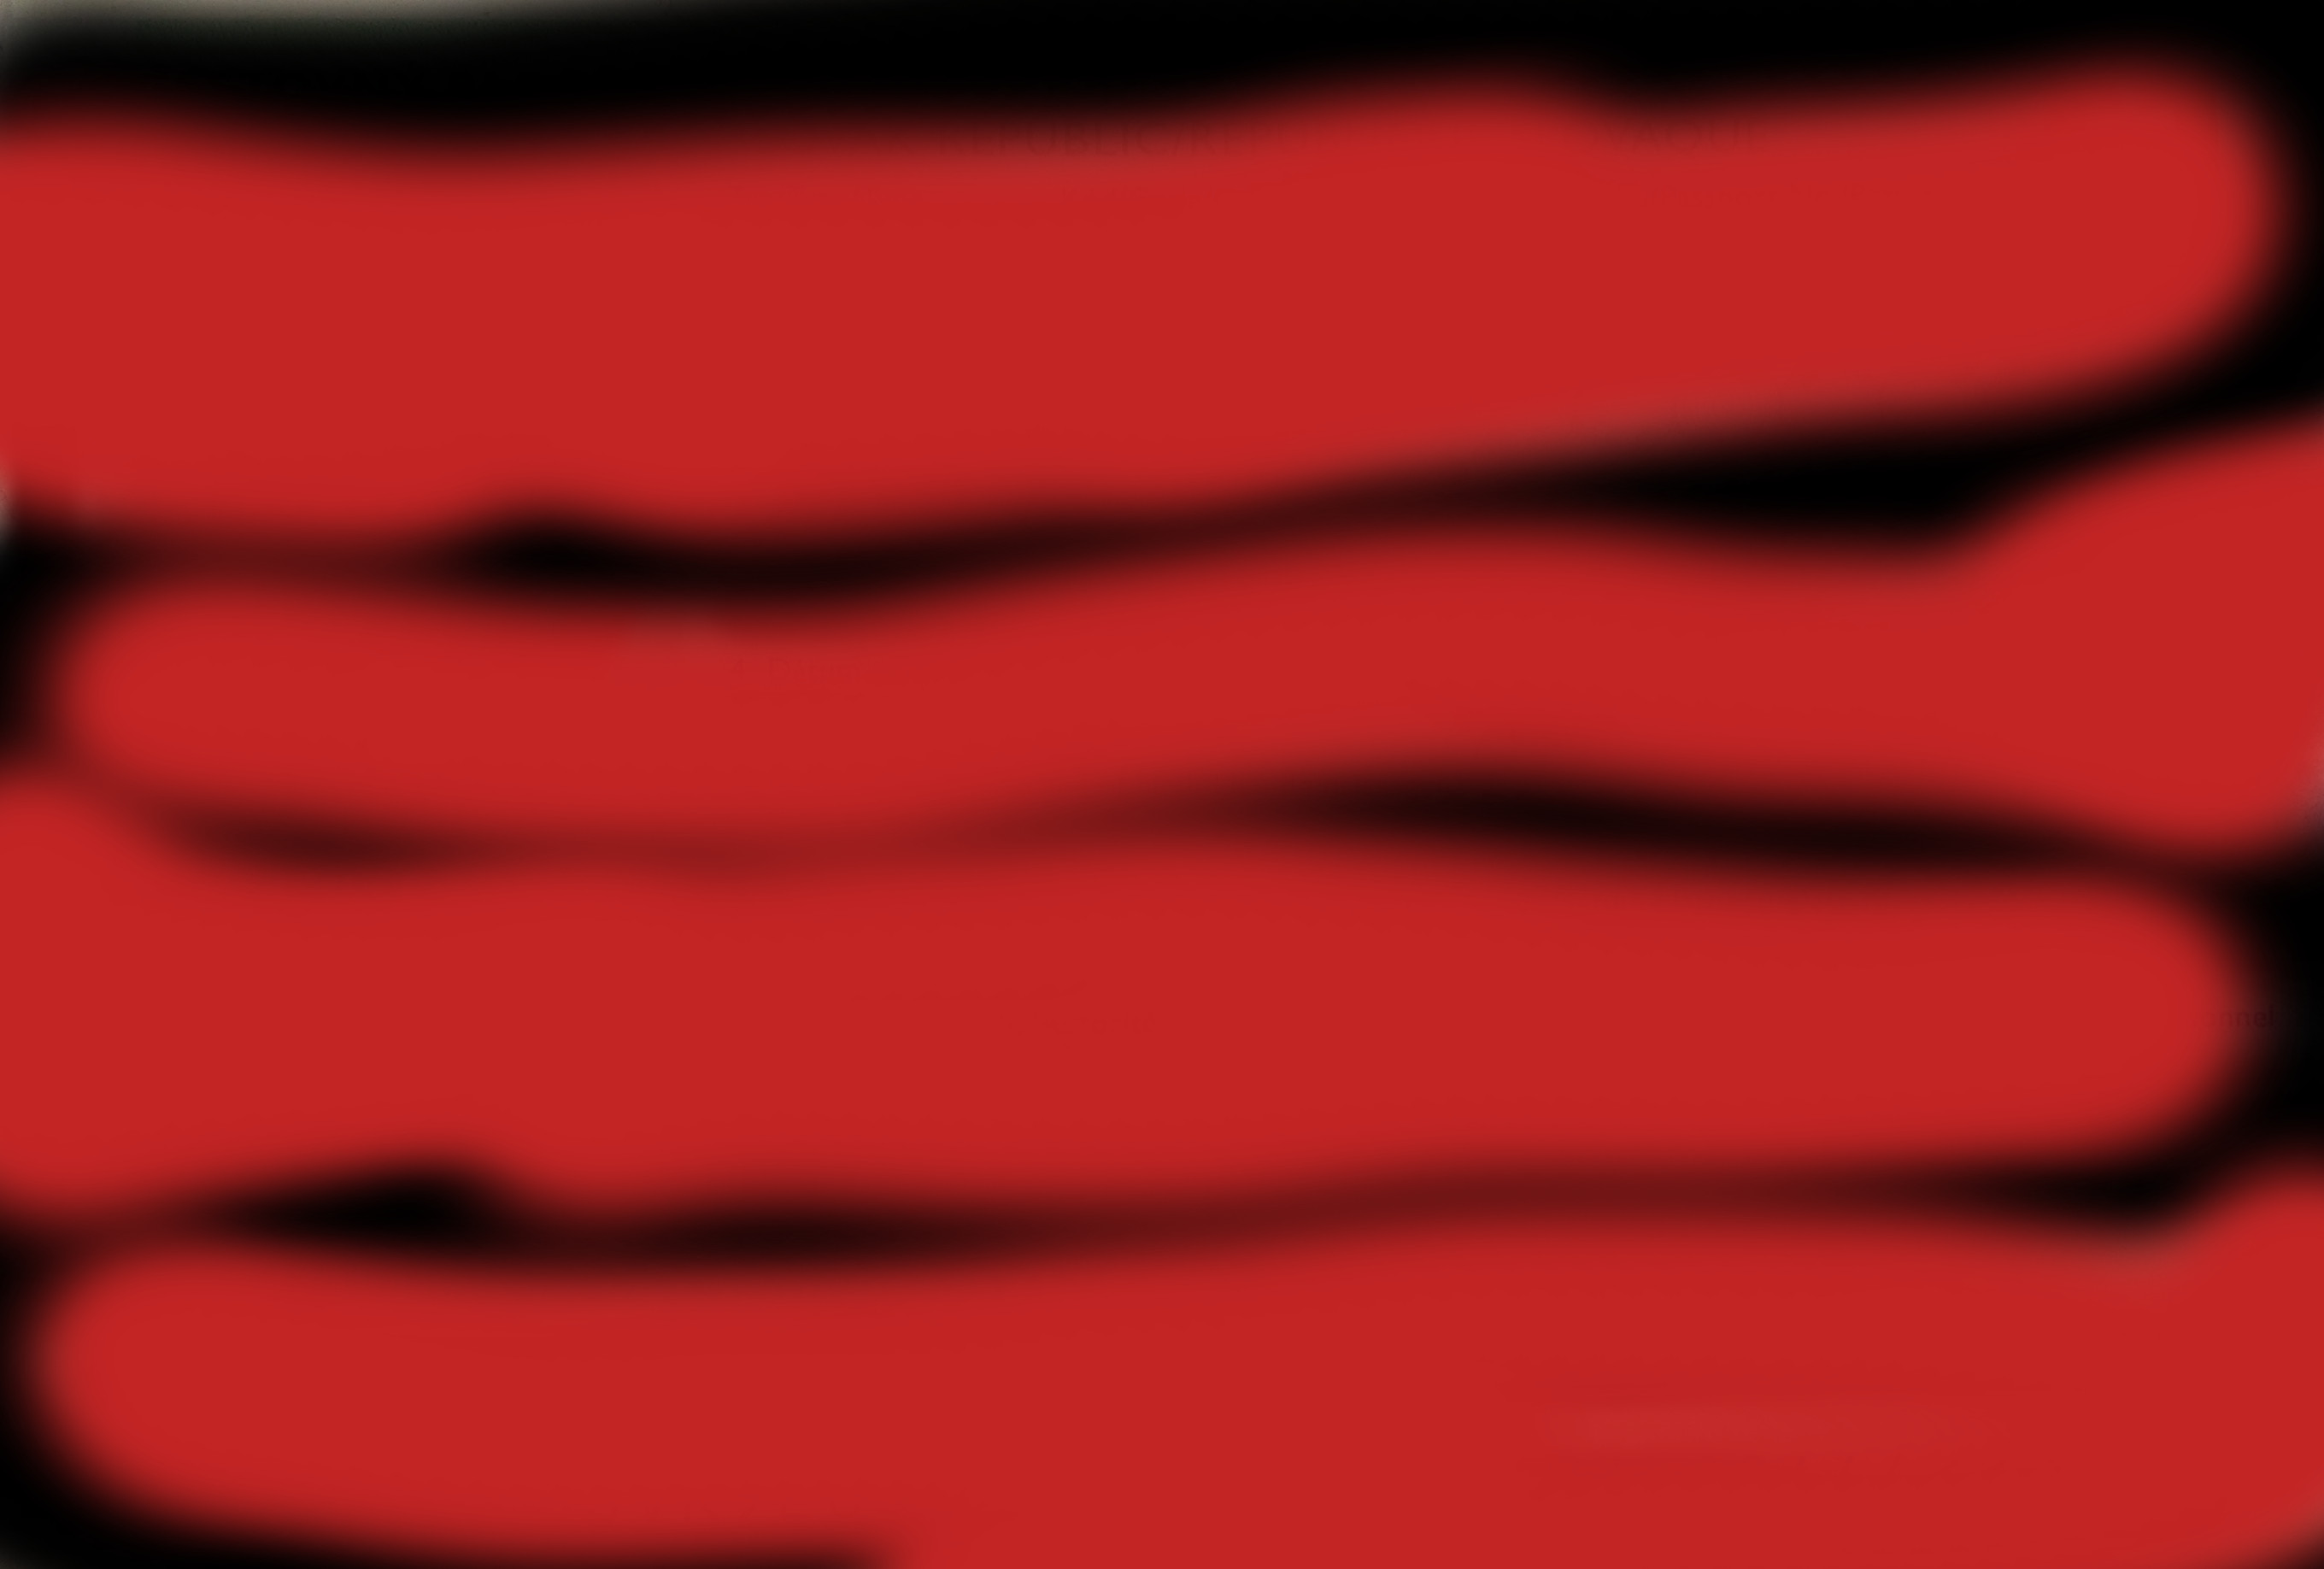
\includegraphics[width=0.8\textwidth]{img/ps.jpg}
\caption{Possible neighborhood functions \cite{Ho03} }
\label{fig:gb}
\end{figure} 	
	
	
\end{introduction}

\setsecnumdepth{all}

\chapter{Probabilistic Models}

Before we start to talk about Continuous-time Hidden Markov Model (CT-HMM), we will briefly explain its discrete-time variant, usually just referred to as Hidden Markov Model (HMM or DT-HMM), starting by explaining the underlaying Markov process. We find it as logical hierarchy as the CT-HMM is the natural extension of the discrete model, sharing many ideas and subroutines and Markov process is the base building block of overall model. The main reference for the DT-HMM was the tutorial article \cite{Ra89}, where more detailed descriptions and examples can be found. The CT-HMM is like the one described in article \cite{Li15}.

\section{Discrete-time Markov Process}\label{sec:DMP}
    
Discrete-time Markov process (also referred to as Markov chain) \cite{TODO} is the stochastic process $X_t$ in discrete equidistant time $\matr{T} = \{ 0, 1, 2, \dots \}$, that in every time-step occupies some state of the potentially infinite state set. However, later in the text, we will consider restricted definition for the finite state sets $\mathcal{S} = \{ s_1, s_2, \dots, s_n\}$.  The process being in time $t_i$ in the state $s_j$ will be denoted as $X_{t_i} = s_j$. The state of the process can change in every time-step. The probability that the process changed from the state $s_i$ to the state $s_j$ is called transition probability. We will refer to it as $a_{ij}$. The transition probabilities for all pairs of states can form the square matrix of size $n$ - transition probabilities matrix $\matr{A}$ . Note that the elements on its diagonal, although referred to as transition probabilities, represent the probabilities of the process remaining in the same state.

The Markov process is memory-less, not holding the information about the past states. So the probability of transition depends only on the current state and is defined in the matrix $\matr{A}$. This characteristic is called the Markov property and can be expressed in the following equation \eqref{eq:mp}.

\begin{equation}\label{eq:mp}
\begin{aligned}
\mathrm{P}(X_t & = s_j \mid X_{t-1} = s_i, X_{t-2} = s_k, \dots)  \\   
               & = \mathrm{P}(X_t = s_j \mid X_{t-1} = s_i ), \quad s_i,s_j,s_k \in \mathcal{S}, t \in \matr{T}
\end{aligned}
\end{equation}

If not stated differently, we will always refer to the time-homogeneous Markov processes. Homogeneity of the Markov process, described in equation \eqref{eq:homo} guarantees that the one step transition probabilities are not changing throughout the time, so the matrix $\matr{A}$ stays constant. 

\begin{equation}\label{eq:homo}
   a_{ij} = \mathrm{P}(X_t = s_j \mid X_{t-1} = s_{j-1} ),\qquad 1 \leq i,j \leq n, \forall t
\end{equation}

For the transition probabilities apply standard stochastic constrains \cite{Ra89}.

\begin{equation}
   a_{ij} \geq 0
\end{equation}

\begin{equation}
   \sum_{j=1}^n a_{ij} = 1
\end{equation}

\section{Discrete-Time Hidden Markov Model}

The Discrete-time Hidden Markov Model (HMM) is the doubly embedded stochastic process consisting of underlaying Markov process $X_t$ \ref{sec:DMP} and another process $O$. The process $O$ assigns to every state $s_i$ the specific observation symbol from the set $\mathcal{V}$ that will be emitted with certain probability. The model is called "hidden", because the state sequence of Markov process is not directly visible. It can only be guessed from statistic over the model parameters. The set $\mathcal{V}=\{  v_1,v_2,\dots,v_m\}$ is the set of all observable (emission) symbols. The probability that the state $s_i$ emits the symbol $v_j$ will be denoted as $b_i(j)$ and together with other elements form the matrix $B$, the rectangular matrix of $n$ rows and $m$ columns. Comparing to the single Markov process, HMM is able to model more complex systems, that can often be close to describe the processes of the real life problems.  
  
The following parameters are needed to describe the HMM:

\begin{enumerate}[resume]
\setcounter{enumi}{0}
\item \textbf{Hidden States}
\begin{equation}
\mathcal{S} = \{ s_1,s_2, \dots, s_n \}
\end{equation} 
\item \textbf{State Transition Probability Matrix}
\begin{equation}\label{eq:tp}
\matr{A} = \{ a_{ij} \}, \quad 1 \leq i,j \leq n
\end{equation} 
\item \textbf{Observation Symbols}
\begin{equation}
\mathcal{V} = \{ v_1,v_2, \dots, v_m \} 
\end{equation}
\item \textbf{Observation Symbols Probability Matrix} \\
$\matr{B} = \{ b_{i}(k) \}$, where $b_{i}(k)$ is the probability that the observation $v_k$ will occur, if the system is currently in state $i$. 
\begin{equation}
b_i(k) = \mathrm{P}(v_k \text{ observed at time }t \mid X_t = s_i), \qquad 1 \leq i \leq n, \quad 1 \leq k \leq m
\end{equation}
\item \textbf{Initial state distribution} \\
$\pi = \{ \pi_i \}$, where $\pi_i$ is the probability of the initial state being $s_i$.
\begin{equation}
\pi_{i} = \mathrm{P}(X_0 = s_i), \qquad 1 \leq i \leq n
\end{equation}
\end{enumerate}

For the convenience we will declare parameter $\lambda = (\matr{A},\matr{B},\pi)$, compactly denoting the set of all parameters of the model. 

\section{Continuous-Time Markov Process}\label{sec:ctmp}

In the discrete-time Markov process described in section \ref{sec:DMP}, the change of the current state of the process could only occur once we have moved a step further in the discrete time $t$. Comparing to this, in the continuous-time Markov process can the change of state occur at any moment in time (the occurrence holds exponential distribution ).

%cit:[S.Karlin]
A finite state continuous-time Markov process is a~stochastic process $\{ X_t \mid t > 0\}$ on the states $\mathcal{S} = \{ s_1, s_2, \dots, s_n \}$  (for $n>0$ and $\mathcal{S}$ being the finite state set), that in any time $t$  occurs in the corresponding state $1 \leq x_t \leq n$. 

For the times $0 \leq u_0 < u_1 < \dots < u_r < u$ it satisfies the following equations: 
\begin{description}
\item [Markov property:] Probability of transition from state $i$ to state $j$ during the time interval $t$ is stationary i.e. independent on the states of process in the times $< u$.  
    
\begin{equation}
\begin{aligned}
& \mathrm{P}( X_{t+u} = s_j \mid X_u = s_i, X_{u_r} = s_{i_r}, \dots , X_{u_0} = s_{i_0} ) = \\ 
& = \mathrm{P}( X_{t+u} = s_j \mid X_u = s_i ), \qquad s_i,s_j,s_{i_0}, \dots ,s_{i_r} \in \mathcal{S} 
\end{aligned}
\end{equation}

The property describes that the stochastic process is memoryless.

\item [Homogeneity:] Probability of transition from the state $s_i$ to $s_j$ in any given time $u \geq 0$ depends only on the length of the time interval $t \geq 0$. 

\begin{equation}
\begin{aligned}
& \mathrm{P}( X_{t+u} = s_j \mid X_u = s_i ) = \mathrm{P}( X_t = s_j \mid X_0 = s_i ) = \\
& = \mathrm{p_{ij}}(t)
\end{aligned}
\end{equation}

\end{description}
 

The upper mentioned conditions assert, that the transition probability $\mathrm{p_{ij}}(t), s_i,s_j \in \mathcal{S}$ satisfies following conditions:%cit:[S.Karlin]


\begin{equation}
\mathrm{p_{ij}}(t) \geq 0
\end{equation}

\begin{equation}
\sum_{j = 1}^n \mathrm{p_{ij}}(t) = 1
\end{equation}

\begin{equation}\label{eq:l0}  
\lim_{t \to 0^+} \mathrm{p_{ij}}(t)= 
\begin{cases}
1, i = j\\
0, i \neq j
\end{cases}
\end{equation}

\begin{equation}\label{eq:ckeq}
\sum_{k = 1}^n\mathrm{p_{ik}}(u)\mathrm{p_{kj}}(t) = \mathrm{p_{ij}}(u+t)     
\end{equation}

Equation \eqref{eq:ckeq} is known as \textit{Chapman-Kolmogorov equation}. 
We can define the matrix $\matr{P_t}$, where the entry $(i,j)$ is $\mathrm{p_{ij}}(t)$ to get the equation in following form:

\begin{equation}\label{eq:ckm}
\matr{P_u} \matr{P_t} = \matr{P_{u+t}},   \qquad t,u > 0  
\end{equation}

\subsection{ Jump Rates }

Using the \textit{Chapman-Kolmogorov equation} \eqref{eq:ckeq}, if we know the probability $\mathrm{p_{ij}}(t)$ for every states $i,j$ and time $0 < t < t_0$, we are able to compute the values for any time $t > 0$. 
%cit[vytistena st. kniha]

The property \eqref{eq:l0}  asserts that $\mathrm{p_{ij}}(t)$ is continuous for $t=0$. It can be showed from equation \eqref{eq:ckm}, after assigning $t=0$ we will get identity matrix $\matr{P_0} = \matr{I}$.
Moreover from \eqref{eq:ckm} follows that $\mathrm{p_{ij}}(t)$ is continuous for all $t>0$ ref[S.Karlin] and so that there exists the right derivative in 0. This knowledge enables us to determine the $\mathrm{p_{ij}}(t)$ for any given time $t>0$.   

\begin{equation}
q_{ij} =  \left.\frac{\mathrm{d}\mathrm{p_{ij}}(t)}{\mathrm{dt}} \,\right|_{t=0} = \lim_{t \to 0^+} \frac{\mathrm{p_{ij}}(t)}{t}, \quad \text{if } i\neq j     
\end{equation}

We will call this derivative $q_{ij}$ the jump rate from state~$i$ to some other state~$j$. The jump rate $q_{ii}$ can be derived from the equation of transition probabilities summing to the one.

\begin{equation}
1 = \mathrm{p_{ii}}(t) + \sum_{j = 1}^{ n ,j \neq i} \mathrm{p_{ij}}(t) 
\end{equation}

dividing by time interval $t$ and letting $t$ decrease close to zero, we will obtain the following equation. 

\begin{equation}\label{eq:qii}
 q_{ii} =  - \sum_{j = 1}^{ n ,j \neq i} q_{ij} 
\end{equation}

(We assume the finite rates $q_{ij}$, infinite rate would immediately lead to the leaving of the state, so it makes no sense for us to consider.)

It can be shown that by construction of the CTMC from discrete time Markov chain (DTMC) and  it's underlying Poisson process with rate $\lambda$, the equation $q_{ij} = \lambda a_{ij}$ holds. Where $a_{ij}$ is the transition probability from the $i$ to $j$ in DTMC \ref{eq:tp}. This is why we call the $q_{ij}$ the jump rate.[zdroj]  

%ROUTING MATRIX - u(i, j) = q(i, j) / lambda max
%u(i, i) = 1 - sum_j u(i, j)

We can also look at $q_{ii}$ as at the rate in which the $X_t$ is leaving the state $i$ \eqref{eq:ckeq}. Then we can define the jump rates matrix $\matr{Q}$ as following:

\begin{equation}
\begin{aligned}  
\matr{Q}(i,j)= 
\begin{cases}
\qquad q_{ij}, \qquad & \text{if } i\neq j\\
\sum\limits_{k = 1}^{ n ,k \neq i} q_{ik}, \qquad & \text{if } i=j
\end{cases}
\end{aligned}
\end{equation}

We can get the transition probabilities for any time $t$ from matrix $\matr{Q}$ by solving the \textit{Kolmogorov's Backward Equation} \eqref{eq:kbe}. It can be obtained from \textit{Chapman-Kolmogorov equation} \eqref{eq:ckm} by differentiation. The solution of the differential equation leads to matrix exponentiation \eqref{eq:mexp}. [zdroj na riesenie]  

\begin{equation}\label{eq:kbe}
\matr{P_t^{'}} = \matr{Q} \matr{P_{t}}
\end{equation}

\begin{equation}\label{eq:mexp}
\matr{P_{t}} = e^{\matr{Q}t}  
\end{equation}

%Such a defined matrix will hold $\pi\matr{Q} = 0$... [explain more, proof, $e^{\matr{Q}t}$]

\subsection{Construction from Discrete-Time Markov Process with Poisson Process Timing } 

The useful way for understanding of the continuous-time Markov process is to know its relation to the discrete process, that can be shown by the construction.

We will take the homogeneous Poisson process $N(t)$ with parameter $\lambda$ and the discrete-time Markov process $Y_{\nu}$, with the states transition probabilities $a_{ij}$. We will assume the $N(t)$ and $Y_{\nu}$ being mutually independent. By changing the equidistant timing of $Y_{\nu}$ to Poisson process timing. We will get the process $Y_{N(t)}$ in which the transition from the state $s_i$ happens at each arrival in $N(t)$ with the probability $a_i = \sum_{j = 1}^{ n ,j \neq i} a_{ij}$ (notice that the transition will not occur if $i=j$). Similarly, the time spent in the state $s_i$ can be described by probability density function of exponential distribution with the parameter $a_i$, $\mathrm{f}(t)= a_i e^{-a_i t}$. Such a process $X_t = Y_{N(t)}$ is called continuous-time Markov process.

Now we can derive the equation for probability of transition from the state $i$ to the state $j$ in the time $t$ as the sum of all the possible number of steps in which the transition can occur. 

\begin{equation}
\begin{aligned}
\mathrm{p_t(i,j)} &= \sum_{n=0}^{\infty} \mathrm{P}( N(t) = n, X_t = s_j \mid X_0 = s_i )  = \\
                  &= \sum_{n=0}^{\infty} \mathrm{P}( N(t) = n, Y_{N(t)} = s_j \mid Y_{N(0)} = s_i )  = \\
                  &= \sum_{n=0}^{\infty} \mathrm{P}( N(t) = n ) \mathrm{P}( Y_n = j \mid Y_0 = i )  = \\
				  &= \sum_{n=0}^{\infty} e^{-\lambda t} \frac{ (\lambda t)^n}{n!} a_{ij}^n  
\end{aligned}
\end{equation} 




\subsection{ Fully Observable Continuous-Time Markov Process }
%ref Yu-Ying Liu

Let's have continuous time Markov process on the state space $\mathcal{S}$, with the jump rates in the matrix $\matr{Q}$, initial state probability distribution $\pi$ and the known hidden state sequence $\matr{X^{'}}= ( x_0^{'}, x_1^{'}, \dots, x_{\nu^{'}}^{'} ) $ occurring with transitions in times $\matr{T^{'}} = ( t_0^{'}, t_1^{'}, \dots, t_{\nu^{'}}^{'} )$. Such a system, where we know, when and where the transition will happen is called fully observable and we can count its complete likelihood ($\mathcal{L}_{FO}$). 

\begin{equation}\label{eq:CL1}
\begin{aligned}  
 \mathcal{L}_{FO} &=  \prod_{u=0}^{\nu^{'}-1} ( q_{x_u^{'} x_{u+1}^{'}} / q_{x_u^{'}} )( q_{x_u^{'}} e^{ - q_{x_u^{'}} \tau_{u }^{'}}) = \\
    &= \prod_{u=0}^{\nu^{'}-1} q_{x_u^{'} x_{u+1}^{'}} e^{ - q_{x_u^{'}} \tau_{u}^{'}}
\end{aligned}
\end{equation}

where the $q_i = \sum_{j=1}^{n,i\neq j} q_{ij}$ is the probability of transition from the state~$i$ and   
$\tau_{u}^{'} = t_{u+1}^{'} - t_{u}^{'}$ is the time interval among the two consecutive steps.

The equation can be further rearranged in the form that group together the same state transition. The variable $\eta_{ij}$ marks the number of transition $q_{ij}$ that have occurred and the~$\tau_i$ is the total time spend in the state~$s_i$.

\begin{equation}\label{eq:CL2}
 \mathcal{L}_{FO} = \prod_{i=1}^{n} \prod_{j=1}^{n, i \neq j} q_{ij}^{\eta_{ij} } e^{ - q_i \tau_i }
\end{equation}

\subsection{ General Continuous-Time Markov Process }

In general we do not know the states of the system during all the time. It is only known at some unevenly distributed times of observations $\matr{T} = ( t_0, t_1, \dots, t_{\nu} )$ as $\matr{X}= (x_0, x_1, \dots, x_{\nu} )$. 
This add an amount of insecurity in the probability computation. We do not longer know, the number of transitions $\eta_{ij}$ as well as the time spend in the specific state $\tau_i$. 

To count the likelihood of the process, we will use earlier defined matrix $\matr{P}(t)$ and its elements $\mathrm{p_{ij}}(t)$ \ref{sec:ctmp}. The time interval among two observation will be marked as  $\tau_u = t_{u+1} - t_u$.    

\begin{equation}
 \mathcal{L} = \prod_{u=0}^{\nu-1} \mathrm{p}_{x_u x_{u+1}}(\tau_u) 
\end{equation}

It can be alternatively extended in the form

\begin{equation}
 \mathcal{L} = \prod_{u=0}^{\nu-1} \prod_{i=0,j=0}^{n}  \mathrm{p}_{ij}(\tau_u)^{\mathbb{I}( x_u = s_i, x_{u+1} = s_j )} 
\end{equation}

where the function $\mathbb{I}(i,j)$ equals either $1$, if both condition inside are true, or $0$ if they are not. 
We will define the $r$ as the number of all distinct time intervals from the set $ \matr{T}_{\Delta} = \{ \tau_1,\tau_2,\dots,\tau_r\}$. If $r$ is lower then the number of observations, it can be beneficial to aggregate them as in formula

\begin{equation}\label{eq:CTL}
 \mathcal{L} = \prod_{\Delta = 1}^{r} \prod_{i=0,j=0}^{n}  \mathrm{p}_{ij}(\tau_{\Delta})^{\mathbb{C}( \tau=\tau_{\Delta}, x_u = s_i, x_{u+1} = s_j )} 
\end{equation}

,where function $\mathbb{C}$ denotes the total number of intervals, for which is the condition true.
    
%TODO P_{ij}(t) counting possibilities.

\section{Continuous-Time Hidden Markov Model}

%The actual state remained hidden, but it has always emitted the observable variable $v_i$.

 %Also it may not be documented by the observation. The emission of the observable variable can happen at any time, however it is independent on the state transition times. For example, it could be times, when the patient undergoes medical examination. The times can generally have highly irregular and unbalanced distribution.

Continuous-time hidden Markov model is the extension of CTMC, where the states in times $\matr{T} = ( t_0, t_1, \dots, t_{\nu} )$ are not directly observed, just seen as the observation symbols sequence $\matr{O} = (  o_0, o_1, \dots, o_{\nu} )$, emitted by the current state $s_i$ with the probability $b_i(o)$.
The likelihood of the completely observed system  $\mathcal{L}_{FO}$ will be similar to the $\mathcal{L}_{FO}$ of CTMC \eqref{eq:CL1} \eqref{eq:CL2} with the difference we need to take into account the probability of actual observation.

\begin{equation}\label{eq:HMCL1}
\begin{aligned}  
 \mathcal{L}_{FO} &= \prod_{u^{'}}^{\nu^{'}-1} q_{x_{u^{'}} x_{u^{'}+1}} e^{ - q_{x_{u^{'}}} \tau_{u^{'}} } 
    \prod_{u=0}^v b_{ x_u }(o_u) = \\
    &= \prod_{i=1}^{n} \prod_{j=1}^{n, i \neq j} q_{ij}^{\eta_{ij} } e^{ - q_i \tau_i } \prod_{u=0}^\nu b_{x_u}(o_u)
\end{aligned}
\end{equation}

There is much more latent information in such defined model. Not just the hidden states, but also the unknown transition times and unknown state sojourn time (how long will the system remain in the state).
Sometimes the state can change, without emitting a single observation. The large number of hidden information make it to be more complex problem then the discrete time model.

\chapter{Statistics}


\section{Expectation-Maximization Algorithm}\label{ch:EM}


%(1) Maximum Likelihood from Incomplete Data via the EM Algorithm , A. P. Dempster; N. M. Laird; D. B. Rubin, Journal of the Royal Statistical Society. Series B (Methodological), Vol. 39, No. 1. (1977), pp.  1-38.

Expectation-Maximization (EM) Algorithm (first introduced in [1]) is the method for finding the Maximum likelihood estimates(MLE) of parameters in probabilistic models over the incomplete data-set ( i.e. data-set containing unobserved (latent) variables ). It is a natural generalization of maximum likeli-
hood estimation, however the latent variables make finding of the MLE more difficult. Direct count can be very computationally expensive, so the EM algorithm uses the iterative approach to approximate the solution by repeating the sequence of simpler consecutive steps.

Let's define vector $\mathbf{x} = (x_{1},x_{2},\dotsc,x_{n})$ containing the known (observed) variables and vector $\mathbf{z} = (z_{1},z_{2},\dotsc,z_{n})$ containing latent (unobserved) variables. We will set $\theta$ for the unknown parameters we want to estimate. We will use the notation $\mathrm{logP}(\mathbf{x},\mathbf{z};\theta)$ as the log-likelihood function, which estimates the probabilities for the given parameters. Notice that we are using the log-likelihood to avoid underflow of parameters values that could otherwise easily arise during the computation.  
%[st]simle tutorial: What is the expectation maximization algorithm? Chuong B Do & Serafim Batzoglou

Look at [st] for more detailed, easily understandable tutorial with examples.    

\begin{enumerate}
\item \textbf{Initialization:} We will make the initial guess of the parameters $\hat \theta_{0} $.
\end{enumerate} 

We will continue by iterating through two following steps: 

\begin{enumerate}[resume]
\item \textbf{Expectation:} Calculate the expected value of the likelihood function $\mathrm{logP}(\mathbf{x},\mathbf{z};\hat \theta_{t})$. Where $\hat \theta_{0}$ is the current parameters estimation. We will find the function $\mathrm{Q}$ that lower bounds $\mathrm{logP}(\mathbf{x},\mathbf{z};\hat \theta_{t})$.

\begin{equation}\label{eq:exp}
 \mathrm{Q}(\hat\theta_{t}) =  \mathrm{logP}(\mathbf{x},\mathbf{z};\hat \theta_{t})
\end{equation}

\item \textbf{Maximization:} Find the value $\hat\theta_{t+1}$ that maximize $\mathrm{Q}(\hat\theta_{t})$.  
\end{enumerate}  

As the value of $\mathrm{Q}(\hat\theta_{t})$ matches the log-likelihood function at $\hat\theta_{t}$, it follows that $ \mathrm{Q}(\hat\theta_{t}) =  \mathrm{logP}(\mathbf{x},\mathbf{z};\hat \theta_{t}) \leq \mathrm{Q}(\hat\theta_{t+1}) =  \mathrm{logP}(\mathbf{x},\mathbf{z};\hat \theta_{t+1}) $ thus the function values in consecutive iterations form the non-decreasing sequence. The computation can be stopped once the parameters converge to some values, that are not changing anymore.  

It is important to notice that this approach may lead to the local optima. To get better results the algorithm can be launched more times, starting always from different randomly initiated parameters. Possibly enhanced by the use of some more advance non-linear optimization technique.

\section{Discrete-Time Hidden Markov Model}\label{sec:3p}
% citate: Jack Ferguson of IDA in lectures at Bell laboratories
When dealing with HMM real-world application we need to deal with following problems [citace]. First we will describe tham and later in the successive subsections we will explain the algorithms that can effectively solve them. 

\begin{enumerate}
\item Compute the probability $\mathrm{P}(\matr{O}|\lambda) $ of the observation sequence \\ $\matr{O} = (o_1,o_2,\dots,o_{\nu})$, given the set of parameters $\lambda = \{A,B,\pi\}$. Elements of the observation sequence $\matr{O}$ are some specific measured data, taking values from the set~$\mathcal{V}$. \label{it:p1}  
\item Choose the optimal state sequence $\matr{X} = (x_1,x_2,\dots,x_{\nu}$), having the observation sequence $\matr{O}$ and parameters $\lambda$. \label{it:p2} 
\item Adjust the model parameters $\lambda$ in the way it maximizes the probability of observation sequence $ \mathrm{P}(\matr{O}|\lambda) $. \label{it:p3} 
\end{enumerate}


\subsection{Forward-Backward Algorithm}\label{sec:fb}
The \textit{forward-backward} algorithm is actually the pair of two separate algorithms (forward vs. backward). We will explain the \textit{forward} one and at the end we will describe the modifications that are needed to do the \textit{backward}. Both of them are sufficient to solve the first proposed problem \ref{it:p1} separately, however we need to define both, because of the use in the later text.  

Forward algorithm is the dynamic programming algorithm benefiting from the Markov property \eqref{eq:mp} - the independence upon past events. We will define the forward variable $\alpha_t(i)$ as the probability of the partial observation sequence, with the last observation in the time $t$ emitted by the state $s_i$, given the model parameters $\lambda$.

\begin{equation}
\alpha_t(i) = \mathrm{P}(o_1,o_2,\dots,o_t,X_t = s_i \mid \lambda )
\end{equation}

The forward variables can be gradually counted using the bottom-up strategy following equations for $t=1$ and $t=t+1$.

\begin{equation}
\alpha_1(i) = \pi_i b_i(o_1), \qquad 1 \leq i \leq n
\end{equation}

\begin{equation}
\begin{aligned}
\alpha_{t+1}(i) = \left( \sum_{j=1}^n \alpha_t(j) a_{ji} \right) b_i(o_{t+1}), \qquad 1& \leq t \leq \nu - 1, \\ 
                                                                                 1& \leq i \leq n		\end{aligned}
\end{equation}

Now we can obtain the solution of the first problem simply by summing through the all forward variables in the time $\nu$.

\begin{equation}
\mathrm{P}(\matr{O}|\lambda) = \sum_{i=1}^n \alpha_{\nu}(i)
\end{equation} 

Similarly we can define backward variable $\beta_t(i)$ as
\begin{equation}
\beta_t(i) = \mathrm{P}(o_{t+1},o_{t+2},\dots,o_{\nu},X_t = s_i \mid \lambda ) 
\end{equation}
The DP algorithm can be derived analogically as the one for the forward procedure, with the single difference, that it will start counting from the end, so the total probability can be count by summing the backward variables in time $t=1$.

We need to count $n$ variables at each time-step, each of them takes exactly $n$ steps to evaluate. It makes overall complexity $\mathcal{O}(n^2\nu)$.    

\subsection{Individually Most Likely States Sequence}\label{sec:ssp}
There are more ways how we can look at the word "optimal" in the problem two statement \ref{it:p2}. One of the possible approaches is to maximize the expected number of correctly assigned states. To solve it, we need to define the variable determining the probability of being in the specific state in the particular time. We will also call it "single state probability".

\begin{equation}
\gamma_t(i) = \mathrm{P}(X_t = s_i \mid \matr{O},\lambda ) 
\end{equation}

Here we can use already defined forward and backward variables and count the $\gamma_t(i)$ as
\begin{equation}
\begin{aligned}
\gamma_t(i) &= \frac{ \mathrm{P}( X_t = s_i, \matr{O} \mid \lambda )}{ \mathrm{P}( \matr{O} \mid \lambda )} =
               \frac{  \alpha_t(i) \beta_t(i) }{ \mathrm{P}( \matr{O} \mid \lambda )} = \\
            &= \frac{  \alpha_t(i) \beta_t(i) }{ \sum\limits_{j=1}^n \alpha_t(j) \beta_t(j) } 
\end{aligned}
\end{equation}

To get the desired individual most likely state $x_t$, it is enough to find one of the highest probability.

\begin{equation}
x_t = \argmax_{1 \leq i \leq n} \gamma_t(i), \qquad 1 \leq t \leq \nu
\end{equation} 

Applying this algorithm to the whole sequence would lead to the highest expected number of correctly assigned states, however the sequence as a whole can in some cases have very low probability or even not be feasible. This would happen if probability of transition among two consecutive states in the sequence was zero.   
   
\subsection{Viterbi Algorithm} 

Another way how to look on the problem two \ref{it:p2} is to find single most probable state sequence. It means to maximize $\mathrm{P}(\matr{X}\mid \matr{O},\lambda)$, what is equivalent to maximizing of $\mathrm{P}(\matr{X}, \matr{O}\mid\lambda)$.

\textit{Viterbi} algorithm is the dynamic programming algorithm, that similarly to the forward-backward algorithm  benefits from memorylessness of Markov Chain. In DP we can gradually count the variable $\delta_t(i)$, that represents the maximal probability of the state chain from its beginning till the state time $t$, with the state $x_{t}$  being $s_i$.

\begin{equation}\label{eq:delta}
\delta_t(i) = \max_{x_1,x_2,\dots,x_{t-1}} \mathrm{P}( x_1,x_2,\dots, x_t = s_i, o_1, o_2, \dots, o_t \mid \lambda )
\end{equation} 

To get the actual state sequence, we need to store the information about the state in time $t-1$ that has maximized the previous equation \eqref{eq:delta}. We will store it in the array $\psi_t(i)$. Now we can define the initialization of the algorithm as

\begin{equation}
\delta_1(i) = \pi_i b_i(o_1), \qquad 1 \leq i \leq n 
\end{equation}

\begin{equation}
\psi_1(i) = 0 
\end{equation}

and consecutive bottom-up computation as

\begin{equation}
\begin{aligned}
\delta_{t}(i) = ( \max_{ 1 \leq j \leq n } \delta_{t-1}(j)a_{ji} ) b_i(o_{t}), \qquad 2& \leq t \leq \nu, \\
																					   1& \leq i \leq n
\end{aligned}
\end{equation}

\begin{equation}
\begin{aligned}
\psi_{t}(i) = ( \argmax_{ 1 \leq j \leq n } \delta_{t-1}(j)a_{ji} ), \qquad \qquad 2& \leq t \leq \nu, \\
																			       1& \leq i \leq n
\end{aligned}
\end{equation}

Now we can get the searched state sequence probability 

\begin{equation}
\mathrm{P}^* = \max_{1 \leq i \leq n} ( \delta_{t}(i) )  
\end{equation}

and the actual state path $\matr{X}^* = ( x_1^*, x_2^*, \dots, x_{\nu}^*)$ by backtracking

\begin{equation}
x_t^* = \argmax_{1 \leq i \leq n} ( \delta_{t}(i) ),  \qquad t = \nu 
\end{equation}

\begin{equation}
x_t^* = \psi_{t+1}(x_{t+1}^*), \qquad t = \nu-1, \nu-2, \dots, 1  
\end{equation}

The structure of the algorithm is very similar to the Forward-Backward algorithm, so we can easily see its complexity is also $\mathcal{O}(n^2\nu)$.

\subsection{Expectation-Maximization Algorithm}\label{sec:BWA}

There doesn't exist analytic solution for the problem~three \ref{it:p3}. There exist more possible iterative algorithms from which we will describe the expectation-maximization approach~\ref{ch:EM}, based on the classic work of Baum and his colleagues called \textit{Baum-Welch} algorithm[ref]. We will start by defining the variable~$\xi_t(i,j)$ as the probability~of being in the state~$s_i$ in the time~$t$ and in state~$s_j$ in the time~$t+1$, later also referred to as "double state probability". 

\begin{equation}
\xi_t(i,j) = \mathrm{P}( X_t = s_i, X_{t+1} = s_j \mid \matr{O}, \lambda )  
\end{equation}

The probability can be compute using forward-backward variables as follows
 
\begin{equation}\label{eq:xi}
\begin{aligned}
\xi_t(i,j) &= \frac{ \alpha_t(i) a_{ij} b_j(o_{t+1}) \beta_{t+1}(j) }
		   		   { \mathrm{P}( \matr{O} \mid \lambda ) } \\
		   &= \frac{ \alpha_t(i) a_{ij} b_j(o_{t+1}) \beta_{t+1}(j) }
		   		   { \sum\limits_{i=1}^n \sum\limits_{j=1}^n \alpha_t(i) a_{ij} b_j(o_{t+1}) \beta_{t+1}(j) }
\end{aligned}
\end{equation}

Obviously it is in relation with already defined variable~$\gamma_t(i)$ - the probability of being in the state~$s_i$ in the time~$t$.

\begin{equation}
\gamma_t(i) = \sum_{j=1}^n \xi_t(i,j)  
\end{equation}

We can get the expected number of transitions from~$s_i$, when summing~$\gamma_t(i)$ over the time till~$\nu-1$. Similarly we would get expected number of times in~$s_i$, by summing $\gamma_t(i)$ from~$t=1$ till~$t=\nu$. 

\begin{equation}
\mathbf{E}(\text{transitions from $s_i$}) = \sum_{t=1}^{\nu-1} \gamma_t(i)  
\end{equation}

If summing~$\xi_t(i,j)$ over the time, we will get expected number of transitions from $s_i$ to $s_j$, . 

\begin{equation}
\mathbf{E}(\text{transitions from $s_i$ to $s_j$}) = \sum_{t=1}^{\nu-1} \xi_t(i,j)  
\end{equation}

Now we have all what is needed to define the reestimated model~$\hat\lambda=(\hat{\matr{A}},\hat{\matr{B}},\hat\pi)$.

\begin{equation}\label{eq:bwpi}
\hat\pi_i = \gamma_1(i)  
\end{equation}

\begin{equation}\label{eq:bwa}
\begin{aligned}
\hat a_{ij} &= \frac{\mathbf{E}(\text{transitions from $s_i$ to $s_j$})}
				   {\mathbf{E}(\text{transitions from $s_i$})}  \\
		    &= \frac{\sum\limits_{t=1}^{\nu-1} \xi_t(i,j)}{\sum\limits_{t=1}^{\nu-1} \gamma_t(i) }
\end{aligned}
\end{equation}

\begin{equation}\label{eq:bwb}
\begin{aligned}
\hat b_{i}(k) &= \frac{\mathbf{E}(\text{times of visiting $s_i$ and observing symbol $v_k$ })}
				   {\mathbf{E}(\text{times of visiting $s_i$})} \\
			  &= \frac{\sum\limits_{t=1, \text{if } O_t = v_k  }^{\nu} \gamma_t(i)}{\sum\limits_{t=1}^{\nu} \gamma_t(i) } 
\end{aligned}
\end{equation}

The formulas can be interpreted as the steps of EM-algorithm, with the expectation step being the computation of auxiliary function~$Q(\lambda,\hat\lambda)$ and maximization step, the maximization over parameter~$\hat\lambda$. The algorithm will stop ones it is no longer improving (re-estimation doesn't bring higher probability). It is important to notice, that the found solution is the local optimum, the searched space can be very complicated containing many local optima, that's way it can be helpful to start the algorithm more times with different parameter initialization.  


\section{Continuous-Time Hidden Markov Model}

We have introduced the basic problems of DT-HMM at the beginning of the section \ref{sec:3p}. They can be similarly defined for the continuous model. Applying the single change that we do not have just the observation sequence $\matr{O}$, but also the time sequence $\matr{T}$, that we need to care about. The solution for the two first problems as well as a considerate part of the third problem is pretty straight-forward. The discrete-time solutions, just need to be redefined with different transition probability matrix for different interval. It will be discussed in the following subsection \ref{sec:pos}. The EM algorithm for jump-rate matrix estimation is not so straight-forward anymore. We need to care about, what is happening in times between two observations, as it has impact on the results of likelihood counting. The EM algorithm and its variants, will be explained in all the remaining subsections.   

%continuous time Baum-Welch -> citace veci, ktore to robili - DP, spaniely, starsi clanok. + preco je novsi clanok lepsi. ->do uvodu toto.

\subsection{The Posterior State Probabilities}\label{sec:pos}

To count the single and double states probability of the CT-HMM with specified parameters, we do not need to know about the state transition that have occurred in between of the two observations.
If we take just the observation points into the account, we can look on the model as it was the time in-homogeneous DT-HMM. It is the model, in which the state transition probabilities can change in every time-step. We have previously defined the transition probability from state $i$ to the state $j$ in time interval $\tau$ as $\mathrm{p_{i,j}}( \tau ) = e^{ \matr{Q} \tau}$, that can play the role of the transition probabilities matrix $\matr{A}$ in the discrete time in-homogeneous model. For example the probability of the model, with the known states in the observation times can be computed as following

\begin{equation}
\prod_{u=1}^{\nu-1} \mathrm{p_{x_u, x_{u+1}}} (\tau_u) \prod_{u=1}^{\nu} b_{ x_u }(o_u)
\end{equation}

The $\tau_u$ is the time interval $t_{u+1} - t_u$. It should be obvious now, that for the continuous variant of Viterbi and Forward-backward algorithm, we only need to change the state transitions $a_{ij}$ to the time variable~$\mathrm{p_{i,j}}( \tau_u )$.   
Now, we can use the forward and backward variables to count posterior state distribution for the single state  $\gamma_t(i) = \mathrm{P}( x_u = i \mid \matr{O},\matr{T}, \matr{ Q_t } )$ and the two consecutive states $\xi_t(i,j) = \mathrm{P}( x_u = s_i, x_{u+1} = s_j \mid \matr{O},\matr{T}, \matr{ Q_t } )$, in the same way,  as we have done in the discrete model.

\subsection{Soft vs. Hard Method}\label{sec:shm}

The described way for computing the posterior state distribution of hidden states is referred to as the \textit{Soft~method}. Supplementary, there is the \textit{Hard~method}. The \textit{Hard~method} EM algorithm try to maximize the probability of the most likely hidden states sequence. The sequence can be obtained by Viterbi algorithm and than be used "hardly" - just considering the single pair of end states for every time interval, to update the double state probabilities table. Important to notice is that the \textit{Hard method} try to maximize the probability of most likely sequence, instead of maximizing the most likely observed data. [https://arxiv.org/pdf/1312.4551.pdf] So the optimization of the second can possibly be created just as the byproduct. Also there is any guarantee, that the probability of the dataset being generated by the model will be non-decreasing throughout the iterations. Instead we can securely claim, the non-decreasing character of maximal state sequence probability. 


\subsection{Continuous-Time Markov Process EM} 

There is no available analytic maximizer of likelihood function \eqref{eq:CTL}, however it can be estimated iteratively by the EM algorithm proposed in [ref:PhysRevE.76][8yy].  
For the expectation step we will use logarithm of expected complete likelihood function \eqref{eq:CL2}, with the estimated parameter of $\matr{Q}$ in step $t$ noted as $\matr{ \hat Q_t } $.

\begin{equation}\label{eq:EMCL}
 \ln( \mathcal{L}_{FO} ) = \sum_{i=0}^n \sum_{j=0}^{n, i \neq j} \ln( \hat q_{ij}) \mathbf{E}( \eta_{ij} \mid \matr{X}, \matr{ \hat Q_t } ) - \hat q_i \mathbf{E}( \tau_i \mid \matr{X}, \matr{ \hat Q_t } )
\end{equation}

In the maximization step we will take the derivative with respect to $q_{ij}$ and evaluate the new values for $\matr{ \hat Q }$, so that the previous equation was maximized. 

\begin{equation}\label{eq:Qmax}
\begin{aligned}  
\matr{ \hat Q_t }(i,j)= 
\begin{cases}
\frac{ \mathbf{E}(\eta_{ij} \mid \matr{X}, \matr{ \hat Q_t } )}{ \mathbf{E}( \tau_i \mid \matr{X}, \matr{\hat Q_t} ) } & \text{if } i\neq j\\
- \sum\limits_{k=1}^{n,k \neq i} q_{ik}, \qquad & \text{if } i=j
\end{cases}
\end{aligned}
\end{equation}

The remaining non-trivial task is to evaluate $\mathbf{E}( \eta_{ij} \mid \matr{X}, \matr{\hat Q_t} )$ and $\mathbf{E}( \tau_i \mid \matr{X}, \matr{ \hat Q_t } )$. They can be expressed as following sums.


\begin{equation}
\begin{aligned}  
\mathbf{E}(\eta_{ij} \mid \matr{X}, \matr{\hat Q_t} ) &= \sum_{u=0}^{\nu-1} \mathbf{E}(\eta_{ij} \mid x_u, x_{u+1}, \matr{ \hat Q_t } ) = \\
&= \sum_{u=0}^{\nu-1} \sum_{k=0,l=0}^{n} \mathbb{I}( x_u = k, x_{u+1} = l ) \mathbf{E}(\eta_{ij} \mid x_u = k, x_{u+1} = l, \matr{\hat Q_t} )
\end{aligned}
\end{equation}


\begin{equation}
\begin{aligned}  
\mathbf{E}( \tau_i \mid \matr{X}, \matr{\hat Q_t} ) &= \sum_{u=0}^{\nu-1} \mathbf{E}(\tau_i \mid x_u, x_{u+1}, \matr{ \hat Q_t } ) = \\
&= \sum_{u=0}^{\nu-1} \sum_{k=0,l=0}^{n} \mathbb{I}( x_u = k, x_{u+1} = l ) \mathbf{E}(\tau_i \mid x_u = k, x_{u+1} = l, \matr{\hat Q_t} )
\end{aligned}
\end{equation}
   
The Markov property and homogeneity of the Markov process allows to reduce the computation of expected values to all foursomes $i,j,k,l \in S$ for all distinct time-intervals. The ways how to do it will be shown later in the text \ref{sec:endexp}.     
   
\subsection{Continuous-Time Hidden Markov Model EM}

For the EM parameters estimation in DT-HMM, we have used the long known Baum-Welch algorithm \ref{sec:BWA}. We can use the similar approach for the estimation of parameters $\hat \pi$ \eqref{eq:bwpi} and $\matr{ \hat B }$ \eqref{eq:bwb}. We just need to use the different transition probabilities matrix for every different interval as described in subsection \ref{sec:pos}.  

The estimation of the $\matr{ \hat Q }$ can't be inherited from the discrete model in this way, because the state transitions are not dependent on the observation times and there can even be more of them between two consecutive observations. The following method proposed in the article [ref:YuYingLiu], was the first which could efficiently solve the issue.        

The expectation step will be the log-likelihood of the model. Simply just the logarithm of the full observation probability function \eqref{eq:HMCL1}.

\begin{equation}\label{eq:EMCTHMM}
\begin{aligned}  
 \ln(\mathcal{L}_{FO}) &= \sum_{i=1}^{n} \sum_{j=1}^{n, i \neq j} \big( \ln( \hat q_{ij}) \mathbf{E}( \eta_{ij} \mid \matr{O},\matr{T}, \matr{ \hat Q_t } ) - \hat q_i \mathbf{E}( \tau_i \mid \matr{O},\matr{T}, \matr{ \hat Q_t } ) \big) + \\
    &+ \sum_{u=0}^{\nu} \mathbf{E}( \ln( b_{ x_u }(o_u) ) \mid, \matr{O},\matr{T},\matr{\hat Q_t} )
\end{aligned}
\end{equation}

The last part of the equation ,specific for the hidden Markov model, doesn't contain $q$, so the maximization will be the same as in equation for Markov process \eqref{eq:Qmax}. Lack of the direct states observations, makes the computation of the expected values $\eta_{ij}$ and $\tau_i$ more challenging. We need to obtain it just from the knowledge about the emission sequence. First we will derive the formula for the expectation $\mathbf{E}(\eta_{ij} \mid O,T, \hat Q_t )$, which can be expressed as the sum through all the possible state sequences.

\begin{equation} 
\sum_{x_0,\dots,x_\nu} \mathrm{P}(x_0,\dots,x_\nu \mid \matr{O},\matr{T}, \matr{ \hat Q_t }) \mathbf{E}(\eta_{ij} \mid x_0,\dots,x_\nu , \matr{\hat Q_t} )
\end{equation}

The expected value formula can be rewritten as the sum for the partial intervals.  

\begin{equation}
 \sum_{x_0,\dots,x_\nu} \mathrm{P}(x_0,\dots,x_\nu \mid \matr{O},\matr{T}, \matr{ \hat Q_t }) \sum_{u=1}^{\nu-1}\mathbf{E}(\eta_{ij} \mid x_u, x_{u+1} ,\matr{\hat Q_t} )
\end{equation}

Because the Markov condition hold, we can interval-wise divide the complex probability function and for every of the time intervals sum through all the possible states $k,l$ at its edges. 

\begin{equation}
\sum_{u=0}^{\nu-1} \sum_{k=0,l=0}^n \mathrm{P}( x_u = k, x_{u+1} = l \mid \matr{O},\matr{T}, \matr{ \hat Q_t }) \mathbf{E}(\eta_{ij} \mid x_u = k, x_{u+1} = l, \matr{ \hat Q_t } )
\end{equation}

The expected value of sojourn time $\mathbf{E}( \tau_i \mid \matr{O},\matr{T}, \matr{ \hat Q_t } )$ can be derived equivalently to get \eqref{eq:tau}.

\begin{equation}\label{eq:tau}
\sum_{u=0}^{\nu-1} \sum_{k=0,l=0}^n \mathrm{P}( x_u = k, x_{u+1} = l \mid \matr{O},\matr{T}, \matr{ \hat Q_t }) \mathbf{E}(\tau_i \mid x_u = k, x_{u+1} = l,\matr{\hat Q_t} )
\end{equation}

In the subsection \ref{sec:pos}, we have shown, how to count $\mathrm{P}(x_u = k,x_{u+1} = l \mid \matr{O},\matr{T}, \matr{ \hat Q_t })$. The remaining part, the computing of $\mathbf{E}(\eta_{ij} \mid x_u = k, x_{u+1} = l,\matr{\hat Q_t} )$ and $\mathbf{E}(\tau_i \mid x_u = k, x_{u+1}) = l, \matr{ \hat Q_t } )$ will be presented in following to subsections. 

\subsection{The End-State Conditioned Expectations}\label{sec:endexp}

We have previously described, how to use end-state conditioned expectations $\eta_{ij}$ and $\tau_i$ to compute estimation of the jump-rate matrix $\matr{Q}$ by maximizing of its resulting probability \eqref{eq:Qmax}. In this section we will discuss them more deeply and show the possible ways how to compute their values.

The Markov process, we are describing is time-homogeneous. So the time offset at the beginning of the interval is not important and we can anchor it toward zero. The two following expectations are equivalent: $\mathbf{E}(\eta_{ij} \mid x_{t_1} = k, x_{t_2} = l, \matr{ Q } ) = \mathbf{E}(\eta_{ij} \mid x_0 = k, x_{t_\Delta} = l, \matr{ Q } )$, where ${t_\Delta} = {t_2} - {t_1}$. It can help us to save some computations, as we can store the values and reuse them, if needed.

The expectations can be expressed as following integrals [cit: 14 Hobolth].   

\begin{equation}\label{eq:exp1}
\mathbf{E}(\eta_{ij} \mid x_0 = k, x_t = l, \matr{ Q } ) = \frac{ q_{ij} }{ \mathrm{p_{kl}}(t) } 
\int_{0}^{t} \mathrm{p_{ki}}(x) \mathrm{p_{jl}}(t-x) dx
\end{equation}

\begin{equation}\label{eq:exp2}
\mathbf{E}( \tau_i \mid x_0 = k, x_t = l, \matr{ Q } ) = \frac{ 1 }{ \mathrm{p_{kl}}(t) } 
\int_{0}^{t} \mathrm{p_{ki}}(x) \mathrm{p_{il}}(t-x) dx
\end{equation}

We already know the solution of differential equation for counting the jump probabilities $\mathrm{p}(t)$. So we can transform the previously stated integrals to the form as shown in equation \eqref{eq:exp2}. We will denote the integrals as $\tau^{ij}_{kl}$. For the equation \eqref{eq:exp2} it will be similarly $\tau^{ii}_{kl}$. 

\begin{equation}\label{eq:int}
\tau^{ij}_{kl} = \int_{0}^{t} \mathrm{p_{ki}}(x) \mathrm{p_{jl}}(t-x) dx = 
\int_{0}^{t} {e^{\matr{Q}x}}[k,i] {e^{\matr{Q}(t-x)}}[j,l] dx
\end{equation} 

\subsection{Methods to Solve End-State CE }\label{sec:solve}

There exist more ways how to solve the proposed integral \eqref{eq:int}. 

If the matrix is diagonalizable, the closed form can be obtained by \textit{Eigen-decomposition} based algorithm as describe in [yu-ying 8]. However as claimed in [yu-ying], the matrices are not diagonalizable in general. That makes the method often inappropriate for use in Baum-Welch algorithm, because the jump-rate matrices can take general form during the computation process.

The another method of \textit{Uniformization} is based on truncating of infinite sum as described in [yu-ying 9]. The main advantage of the method is that all the matrices can be precomputed and later reused, so it doesn't need any additional matrix multiplication. \ref[yu-ying] The use of hard or soft method \ref{sec:pos} influence the time performance of the algorithm, with hard method being faster, because of the posterior state probability table will become sparse. The method's running time also highly depends on the data and values of $\matr{Q}$ matrix, as the sequence truncating point can differ significantly.         

The method referred to as \textit{Expm} is using \textit{Matrix exponentiation} to count the proposed integrals. The method is described in article [https://www.cs.cornell.edu/cv/ResearchPDF/computing.integrals.involving.Matrix.Exp.pdf]. The advantage is that just by one exponentiation of auxiliary matrix, we can get results for all pairs of $k,l$ end-states expectations. The auxiliary matrix $\matr{W}$ is in the form $\matr{W} =  \begin{pmatrix} \matr{Q} & \matr{I}_{ij} \\ 0 & \matr{Q} \end{pmatrix} $, where $\matr{I}$ is the square matrix of size $\matr{Q}$ composed by zeros and the only one at position $i,j$. $i,j$ refer to the states of intermediate visit, as defined in previous subsections. You can see that following equality holds $ \int_{0}^{t} {e^{\matr{Q}x}}[k,i] {e^{\matr{Q}(t-x)}}[j,l] dx  =  \int_{0}^{t} ( e^{\matr{Q}x} \matr{I} e^{\matr{Q}(t-x)} )[k,l] dx $. In the article [cornell] is shown that $\int_{0}^{t}  e^{\matr{Q}x} \matr{I} e^{\matr{Q}(t-x)} = {e^{\matr{Q}t}}[0:n][n+1:2n]$, where $n$ is the size of the matrix $\matr{Q}$.

We have got the matrix exponential form, for which conventional methods for matrix exponentiation can be used. For example scaling and squaring method, using Pad\'{e} approximants [yu-ying16 djvu].      


\section{Algorithms for CT-HMM parameters estimation}\label{sec:alg}

This section will roughly describe the algorithm for CT-HMM learning - expectation maximization approach estimating the jump-rate matrix $\matr{Q}$ \ref{pe} also denoting as continuous-time Baum-Welch algorithm. We will only show the parts specific for continuous-time model. The estimation of the other parameters ($\matr{\pi},\matr{B}$), forward and backward algorithm, so as the single and double state probabilities can be easily derived from DT-HMM algorithm \ref{sec:3p}. It is also detail described in article [hmm-base].

The base of the algorithm is described in \ref{pe}, reffering to its most important, frame parts.  The algorithm shows training at a single observation and time sequence. It is for the sake of simplicity, the training by more complex dataset can be made by iterating trough all the sequences. There are two methods affecting the way of convergence - \textbf{soft} and \textbf{hard} \ref{sec:shm}. The soft method uses the forward-backward algorithm and the hard uses the Viterbi algorithm to count posterior state probabilities (single and double-state).

The part that counts the end-state conditioned probabilities is described separately and it compounds two variants different by implementation and computational complexity. We refer to them as \textbf{float-interval} variant \ref{fv} (the name is derived from ability of the algorithm to process float time-intervals) and \textbf{integer-interval} variant \ref{iv} ( it can only process the data with integer time intervals). As showed in the experiment chapter, the second mentioned is significantly faster \ref{sec:cc} and it is probably not the cause of any critical progressive numerical errors \ref{sec:ns}.

The both variants of the described algorithms iterate through all the pairs of hidden-states. Namely at $3^{rd}$ line of \textbf{float-interval} \ref{fv}, and at $2^{nd}$ and $5^{th}$ line of \textbf{integer-interval} variant \ref{iv}. It can be optimized for sparse jump-rate matrices $\matr{Q}$. We can simply omit the pairs with zero jump rate, as once being set to zero, the value can't change by the run of the algorithm.       

\noindent\begin{minipage}{\textwidth} 
\renewcommand\footnoterule{}
\begin{algorithm}[H]
\caption{CT-HMM Parameters Estimation}\label{pe} 
\begin{algorithmic}[1]
\State \textbf{Input data:} observation sequence $\matr{O} = (o_1,o_2,\dots,o_{\nu})$, time sequence $\matr{T} = (t_1,t_2,\dots,t_v)$
\State \textbf{Input parameter:} $n$ - number of hidden states
\State \textbf{Output:} $\matr{\hat{Q}}$ - estimation of jump-rates matrix $\matr{Q}$
\Procedure{Baum-Welch}{}
\State $\matr{\hat{Q}} \gets$ randomly generated jump-rate matrix
\State $\matr{T}_{\Delta} \gets$ find all distinct time intervals from $\matr{T}$
\Repeat
\State $\matr{P}({t_{\Delta}}) \gets \text{ count state transition probabilities } e^{\matr{\hat Q}t_{\Delta}} \text{ for each } t_{\Delta} \text{ from } \matr{T}_{\Delta}$
\State $\matr{\Xi} \gets \matr{\Xi}[u,k,l] = \mathrm{P}( X_{t_u} = k, X_{t_{u+1}} = l \mid \matr{O},\matr{T}, \matr{ \hat Q }),  u \in 1,\dots,v-1$
\State \Comment The double state probability can be counted either from \textit{forward} and \textit{backward} probability tables - \textbf{soft} method, or from \textit{viterbi} algorithm most probable state sequence - \textbf{hard} method. The $\matr{P}({t_{\Delta}})$ is used for counting of state transition probabilities. 
\State $\matr{\Xi}_{\Delta} \gets \text{ sum together the matrices } \matr{\Xi}[u] \text{ with the same length of the time interval } t_{u+1} - t_u \text{ that equals } t_{\Delta} \in \matr{T}_{\Delta}, u \in 1,\dots,v-1 $
\State Count end-state probabilities $\mathbf{E}(\eta_{ij} \mid \matr{O}, \matr{T}, \matr{ \hat Q } ) \text{ and } \mathbf{E}(\tau_{i} \mid \matr{O}, \matr{T}, \matr{ \hat Q })$
\State \Comment It can be counted by one of the two \textit{expm} based algorithm variants described later, \textbf{float-interval} \ref{fv} or \textbf{integer-interval} variant \ref{iv}.  
\State $\matr{\hat{Q}} \gets \matr{\hat{Q}}[i,j] = \frac{\mathbf{E}(\eta_{ij} \mid \matr{O}, matr{T}, \matr{ \hat Q } )}{\mathbf{E}(\tau_{i} \mid \matr{O}, matr{T}, \matr{ \hat Q })} \text{, and } \matr{\hat{Q}}[i,i] =  - \sum_{i \neq j} \matr{\hat{Q}}[i,j]$ \footnote{\label{refqmax}\eqref{eq:Qmax}}
\Until{ probability is satisfiable }

\EndProcedure
\end{algorithmic}

\end{algorithm}

\end{minipage}




\begin{algorithm}[h]
\caption{The Expm Based Algorithm for Counting End-States Conditioned Probabilities (Float-Interval variant)}\label{fv}
\begin{algorithmic}[1]
\Procedure{Float-Interval}{}
\ForAll{$t_{\Delta} \in \matr{T}_{\Delta}$}
 \ForAll{$ \text{pair of states } i,j  \in \mathcal{S}$}
	\State $\matr{D}_{ij} \gets (e^{t_{\Delta} \matr{W}}){[0:n][n+1:2n]}\text{, where } \matr{W} = \begin{pmatrix} \matr{Q} & \matr{I}_{ij} \\ 0 & \matr{Q} \end{pmatrix} $
	\State $\matr{D}_{ij} \gets \frac{ \matr{D}_{ij} }{\matr{P}({t_{\Delta}})}$ 
	\If {$i$ is equal to $j$}
	 \State $\mathbf{E}(\tau_{i} \mid \matr{O}, \matr{T}, \matr{ \hat Q }) = \sum_{k,l \in \mathcal{S}} \matr{\Xi}_{\Delta}[t_{\Delta},k,l] \matr{D}_{ii}[k,l]$  
	\Else 
	 \State $\matr{D}_{ij} \gets  \matr{D}_{ij} \matr{Q}{[i,j]}$
	 \State $\mathbf{E}(\eta_{ij} \mid \matr{O}, \matr{T}, \matr{ \hat Q } ) = \sum_{k,l \in \mathcal{S}} \matr{\Xi}_{\Delta}[t_{\Delta},k,l] \matr{D}_{ij}[k,l]$ 
  	\EndIf 
 
 \EndFor
\EndFor
\EndProcedure
\end{algorithmic}
\end{algorithm}

\begin{algorithm}[h]
\caption{The Expm Based Algorithm for Counting End-States Conditioned Probabilities (Integer-Interval variant)}\label{iv}
\begin{algorithmic}[1]
\Procedure{Integer-Interval}{}
 \ForAll{$ \text{pair of states } i,j  \in \mathcal{S}$}
	\State $\matr{D}_{ij} \gets (e^{\matr{W}})_{[0:n][n+1:2n]}\text{, where } \matr{W} = \begin{pmatrix} \matr{Q} & \matr{I}_{ij} \\ 0 & \matr{Q} \end{pmatrix} $
 \EndFor
\ForAll{$t_{\Delta} \in \matr{T}_{\Delta}$}
  \ForAll{$ \text{pair of states } i,j  \in \mathcal{S}$}
    \State $\matr{D}_{ij}^{'} \gets  \matr{D}_{ij}^{t_{\Delta}} $
    \Comment Use \textit{square and multiply} algorithm to effectively compute	power of $\matr{D}_{ij}$. Notice that every $t_{\Delta}$ needs to be integer.
	\State $\matr{D}_{ij}^{'} \gets \frac{ \matr{D}_{ij}^{'} }{\matr{P}({t_{\Delta}})}$ 
	\If {$i$ is equal to $j$}
	 \State $\mathbf{E}(\tau_{i} \mid \matr{O}, \matr{T}, \matr{ \hat Q }) = \sum_{k,l \in \mathcal{S}} \matr{\Xi}_{\Delta}[t_{\Delta},k,l] \matr{D}_{ii}^{'}[k,l]$  
	\Else 
	 \State $\matr{D}^{'}_{ij} \gets  \matr{D}_{ij}^{'} \matr{Q}_{[i,j]}$
	 \State $\mathbf{E}(\eta_{ij} \mid \matr{O}, \matr{T}, \matr{ \hat Q } ) = \sum_{k,l \in \mathcal{S}} \matr{\Xi}_{\Delta}[t_{\Delta},k,l] \matr{D}^{'}_{ij}[k,l]$ 
  	\EndIf 
  \EndFor
\EndFor
\EndProcedure
\end{algorithmic}
\end{algorithm}

\FloatBarrier

\section{Complexity}\label{sec:complex}

\subsection{Time Complexity}

By complexity we will refer to the complexity of one iteration of EM-algorithm. All the iterations are equivalent, so to get full runtime complexity you can multiply by the iteration number.

The number of hidden states will be denoted as $n$, the summary length of the training sequences as $\nu$. 

\begin{itemize}\label{it:dtc}
\item \textbf{ Discrete-Time Baum-Welch Algorithm } \\
In one iteration of the discrete version of the algorithm the following main procedures take part:
\begin{itemize}
\item Forward algorithm - complexity $\mathcal{O}(n^2\nu)$ \ref{sec:fb}.
\item Backward algorithm - complexity $\mathcal{O}(n^2\nu)$ \ref{sec:fb}.
\item Computation of single state probabilities \ref{sec:ssp} - complexity $\mathcal{O}(n\nu)$. Summing and normalizing the forward and backward probabilities, that are of size $n\nu$.
\item Computation of double state probabilities - complexity $\mathcal{O}(n^2\nu)$ \eqref{eq:xi}. Constant-time computation of probabilities for every pair of states in every time.
\item Various summing operation - complexity $\mathcal{O}(n^2\nu)$. Just linear pass trough the arrays, the biggest one has size $n^2\nu$.
\end{itemize}

As the operations are consecutive, the whole asymptotic complexity of the algorithm is the maximum -  $\mathcal{O}(n^2\nu)$.

\item \textbf{ Continuous-Time Baum-Welch Algorithm } \\

The complexity of the continuous-time algorithm depends on the chosen variant of end-state conditioned probabilities counting. So we will distinguish \textit{integer-interval} \ref{iv} and \textit{float-interval} \ref{fv} variant of algorithm (later just algorithm). In the first one is the time difference among two consecutive observations integral, in the second it is float. Float algorithm can be used for the integral intervals, but not vice-versa. 

The \textit{soft} and \textit{hard} method of convergence \ref{sec:shm} doesn't impact the asymptotic complexity, as both forward-backward algorithm and Viterbi algorithm 
have the same $\mathcal{O}(n^2 \nu)$ complexity.

We will define $r$ as the number of different time intervals. In some cases it can be much more restrictive than $\nu - 1$ - the number of all intervals.

The first part of the algorithm is similar to the discrete-time version \ref{it:dtc}. With the difference, that we need to pre-compute the transition probabilities matrix for every time interval. Than we can simply use the discrete-time algorithms, as if dealing with heterogeneous Dt-HMM. 


\begin{itemize}\label{it:ctc}
\item Pre-compute transition probability matrices - complexity $\mathcal{O}(r n^3)$. Call expm algorithm $\mathcal{O}(n^3)$[gmail April 12] for every distinct time interval. %[pozn. ze to ide mozno zrychlit, ale zbytocne]
\item Subpart similar to discrete-time algorithm - complexity $\mathcal{O}(n^2 \nu)$ \ref{it:dtc}.
\item 

Count end-state conditioned expectations \ref{sec:endexp}:
\begin{enumerate}[resume]
\setcounter{enumi}{0}
\item \textbf{integer-interval algorithm}:

\begin{itemize}
\item Preprocessing end-state conditioned expectation - complexity $\mathcal{O}(n^5)$. 
    In this step we compute all the integrals\eqref{eq:int} for unit time interval. It needs to call expm method $\mathcal{O}(n^3)$[gmail] at matrix $\matr{W}$for every $i$ and $j$ \ref{sec:solve}.   
\item Count matrices for every time interval - complexity $\mathcal{O}(r n^5\log(t_{\max}))$, where $t_{\max}$ is the longest time interval among two consecutive observations.

For every time interval, we will go trough $n^2$ matrices, that we have already precomputed and we will count its value for actual interval by using square and multiply approach. 

%[not asymptotically usefull] We can still make better by precomputed intermediate powers of matrices till $t_{\max}$. This will take  out some computation from main cycle and we can obtain the complexity $\mathcal{O}( max( r*n^3*log(t_{\max}), r*n^5*log(t_{\max}) ) )$.

\end{itemize}

\item \textbf{float-interval algorithm}: 
\begin{itemize}
\item Count end-state conditioned expectation for every interval - complexity $\mathcal{O}(r n^5)$. 
We needs to call expm method $\mathcal{O}(n^3)$[gmail] at matrix $\matr{W}t$ for every $i$ and $j$, where $t$ is the length of the interval \ref{sec:solve}.
\end{itemize}
\end{enumerate}
 
\end{itemize}   

The overall time complexity of the iteration is $\mathcal{O}( r n^5 + n^2\nu )$, using the \textit{float-interval} algorithm and $\mathcal{O}( r n^5\log(t_{\max}) + n^2\nu )$ using the \textit{integer-interval} algorithm. However, it doesn't necessary mean the float-algorithm will run faster. As showed in the time measurement experiment \ref{sec:cc}, the multiplicative constant for \textit{expm} algorithm is very high. The experiment has shown, that there also exists logarithmic pseudo-dependence on parameter $t_{\max}$. It is bounded to counting of Pad\'{e} approximants. The matrices containing bigger numbers, in average need to use the approximant of higher order, which is more complex to compute in the terms of multiplicative constant. We have shown, that in the real practice, it is generally much more computationally efficient to use the integer-interval algorithm.

Till now, we have assumed the full jump-rate matrix $\matr{Q}$. However, in some cases we may intentionally forbid some state-to-state transitions. Such a restriction will also manifest itself in the term of complexity. Let's define $m$ as the number of allowed state-to-state transition pairs. Than the new complexity will shrink to $\mathcal{O}( r n^3 m + n^2\nu )$ or $\mathcal{O}( r n^3 m \log(t_{\max}) + n^2\nu )$ respectively. Notice that the possible value for $m$, which is making sense, can be in the interval $[n,n^2]$, depending on the sparsity of the matrix $\matr{Q}$. So it can effectively divide the full matrix complexity by $n$.  

\end{itemize}

\subsection{Memory Complexity}
In the discrete-time algorithm is the biggest array, the one for storing double state probabilities, so the memory complexity is equal to its size - $\mathcal{O}(n^2\nu)$. 

In the continuous time model there are more arrays of size $n^2\nu$ and the array of size $n^4$ to store precomputed matrix exponentials. So the final memory complexity is $\mathcal{O}( n^2\nu + n^4 )$.

\chapter{Implementation}

The chapter discuss chosen technology and specific details of implementation. 
The code, tutorial and documentation to the library can be found in additional materials.

\section{About Library}

The goal was to create the library, that can be used by broad range of users. Such a library should be written in the well known programming language. It should be easy to install and also it should have the introductory tutorial, that will help to get orientation in the most of the library functionality. 

To accomplish the established goal we have chosen to create \textit{Python} library. Specifically, the development was done under \textit{Python 3.5}. The Python is highly used among machine-learning community and the library is easily accessible by downloading from \textit{Pip}. %TODO [link to pip]. 

The continuous-time hidden Markov model parameter estimation is computationally highly demanding. The using of the plain \textit{Python} would make it cumbersome. To deal with the issue, we have used libraries \textit{NumPy} - for effective work with array and matrices and \textit{SciPy} \cite{Sc01} for the implementation of \textit{exmp} algorithm. To make the computational performance even higher, we have decided to code all the most demanding parts in \textit{Cython} [http://cython.org/]. Cython is a compiled language that generates \textit{CPython} extension modules, so that the code-parts written in the language can get \textit{C}-like performance. The advantage is, its easy integration into the Python module.

The best way how to learn to use the library is follow the code examples. That's way we have decided to create \textit{IPython} notebook with library usage examples, covering all the main use-cases of the library. Reading it, the follower can get the understanding how to correctly use the library and learn, what features are supported.          


\section{Logarithmic Probabilities}

The probability values obtained in the hidden Markov models can often get extremely small. Using the standard data-types, it could fast reach the underflow. Even the short sequences of few hidden states can underflow, if proper conditions are met. 

The use of infinite data-type would be possible. However, it would make the algorithm unacceptably computationally and memory expensive, as the bit-length of the numbers can grow linearly with the number of probabilities to multiply.

More appropriate is to use log-probabilities \eqref{eq:logprob}. This will make the numbers grows linearly, thus their bite-length logarithmically. Under this conditions is the underflow for common data types and the feasible size of the data-set almost impossible.

\begin{equation}\label{eq:logprob}
\mathrm{log}(\mathrm{p}_1\mathrm{p}_2) = \mathrm{log}(\mathrm{p}_1) + \mathrm{log}(\mathrm{p}_2)
\end{equation}   

\section{"Log-sum-exp" Trick}

The log-probabilities work great for multiplication and division, but the problem appears, once we need to sum the probabilities. The so called "log-sum-exp" trick can be used to deal with the issue. 

Let's have probabilities $ \mathrm{p}_1, \mathrm{p}_2, \dots ,\mathrm{p}_n $. Now we want to make the sum of them. It is fairly simple, when they are usual float numbers: $\sum_{i=1}^n \mathrm{p}_i$. But it can get trickier, if they are stored in the form of log-probability. We will denote log-probability $\mathrm{log}( \mathrm{p}_i )$ as $a_i$. Than we can write the sum in the following form \eqref{eq:logsum} . Notice that the output is also log-probability.

\begin{equation}\label{eq:logsum}
\mathrm{log} \big( \sum_{i=1}^n e^{a_i} \big)
\end{equation}

We can't count it directly, as the $e^{a_i}$ can be very small and underflow. The idea of the trick is to take the biggest element out of the sum, as a multiplier and move all the other in relative position toward it.
Let's $b = \max_{i} a_i$. Than we can write the previous equation \eqref{eq:logsum} in the form of equation \eqref{eq:logsum2}. 

\begin{equation}\label{eq:logsum2}
\begin{aligned}
&\mathrm{log} \big( e^b \sum_{i=1}^n e^{a_i - b } \big) = \\
 = \quad &  b + \mathrm{log} \big( \sum_{i=1}^n e^{a_i - b } \big)
\end{aligned}
\end{equation}

This approach will only dismiss the elements, that are relatively for data-type maximal-range smaller than the biggest element $b$. You can see, that also the sum of more such diminished elements will, under normal circumstances, never have an impact on the precision of computation - comparing the data-type imprecision.     

%TODO \section{End of Convergence}
%..stop at the end of convergence
%second derivative is not monotonous. 

\section{The Sparse Jump-Rate Matrix}

The time-complexity of the CT-HMM EM algorithm can shrink, when using the sparse matrix \ref{it:ctc}. The implementation take advantage of it, but not in the term of the theoretical complexity, since it is still cycling trough all the matrix elements. The algorithm just stop to perform the body of the cycle. Such solution may seems to be less effective in the terms of theoretical time-complexity. But under the real conditions will be the number of states not bigger than hundreds, so just cycling through all the matrix elements is utterly negligible, comparing the matrix exponentiations taking part in the body of the cycle.   
 
\chapter{Experiments}

The definition of the hidden Markov models may seem to be simple. However, in consequences it covers many non-trivial characteristics that needs some intuition to be understood correctly. This chapter is purposed to discuss such characteristic, and simultaneously try to support the allegations by presenting the experiments.

The later part of the chapter, will contain the experiments, that are in some way connected to the implemented methods or HMM theory. Either comparing the methods or exploring their specific behavior.       

\begin{enumerate}[resume]
\setcounter{enumi}{0}
\item \textbf{Models Convergence Comparison} \\
Compare the discrete and continuous-time HMM at the equivalent dataset.
\item \textbf{Computational Complexity} \\
Examine the time complexity and compare it with theoretical expectations.
\item \textbf{Numerical Stability} \\
Compare the \textit{float-interval} and \textit{integer-interval} method from the point of numerical stability.
\item \textbf{Hidden States Number} \\
Examine behavior of the models trained with different numbers of hidden states.

\end{enumerate}


\section{Models Convergence Comparison}

In the theoretical part, we are describing two models, discrete-time and continuous-time hidden Markov model. The model convergence test will compare, how fast they can learn from generated dataset (converge to the local optima) and we will check, if there is some significant difference among the converged optima values. 

As the continuous-time model takes, except the observations, also the time vectors, its domain range is obviously much broader. Still, it is possible to train it at the dataset for discrete-time model, simply by adding artificial equidistant time vectors.

\subsection{ Description }

For the first experiment we have used the dataset generated by the model, which we have created artificially to suit its purpose well. %TODO See its parameter here [table]. 
The model contains three hidden states and three observation symbols. Comparing the general random generated model, it takes advantage of its more extreme position in the parameter space, so its distance to the most of the random generated parameters is bigger. This makes the problem of convergence harder and in final produces nicer graphs, unfolding more of the process characteristics.
%TODO separate it into two experiments.

In the second experiment, we have repeated the procedure of the first experiment five times on the models, which parameters were created by hand in some specific real-life like manner, and five times with randomly generated models. 

Training dataset consists of 50 vectors, each of them compounding 50 observation. For the continuous-time model we have add the same number of time vectors, with unit time differences.

In the test, we have conducted ten runs of Baum-Welch algorithm, always starting from different random position and averaged the result. The starting positions were equivalent for both models. We have run 150 iterations for every convergence.

You can see the convergence sequences for the single runs of the first experiment in the figure \ref{fig:sr50} and then their average in the figure \ref{fig:avgc}. Figures \ref{fig:all} and \ref{fig:random} show the results of the second experiment. Notice that the \textit{performance ratio} refer to the ratio of the logarithmic probability estimations of the trained model toward the original model (the one, which was used to generate dataset). So the lower the ratio is, the better fit the model the dataset. The performance ratio of the model before the first iteration is cut of the graph, because it often takes too extreme value.

\subsection{ Observations }

In the figures with the average convergences \ref{fig:avgc} and \ref{fig:all} we can see the continuous-time model converge slightly slower. However the both model seem to converge to the same value, closing the gap by every iteration.
 
The single run convergences \ref{fig:sr50} show the irregular speed of convergence of both models. The better performance at the beginning, doesn't ensure, it will not be over-performed by other instances later. The convergence derivation seems to be more regular towards the end of convergence.

The convergences lines to the datasets generated by the random models start mostly with visibly lower performance ratio than the convergence lines generated by specific hand-made models \ref{fig:all}. 

We can also see that the models mostly over-performed the original model. For example, the average convergence from the first experiment \ref{fig:avgc} is converging to the performance ratio $\sim 0.99372$.  

\begin{figure}
\centering
\begin{minipage}{.8\textwidth}
  \centering
  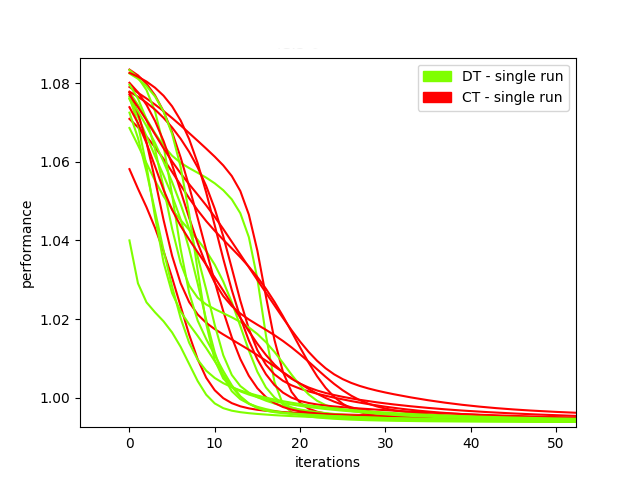
\includegraphics[width=1\linewidth]{img/ex1/1/single_runs_zoom50.png}
  \captionof{figure}{Convergence from various random starting points.}
  \label{fig:sr50}
\end{minipage}
\begin{minipage}{.8\textwidth}
  \centering
  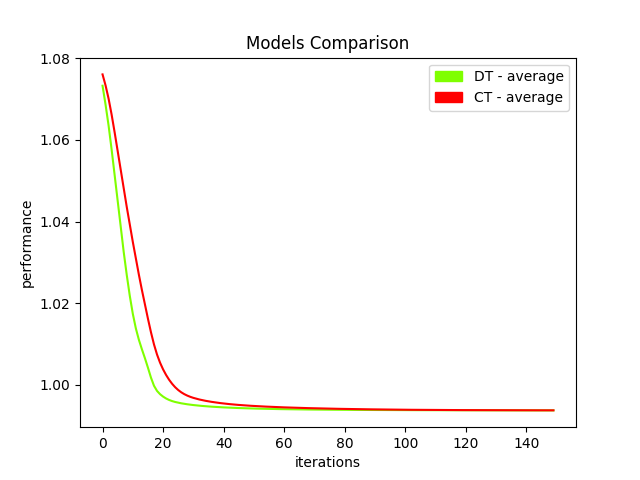
\includegraphics[width=.95\linewidth]{img/ex1/1/average.png}
  \captionof{figure}{Average convergence for various random starting points.}
  \label{fig:avgc}
\end{minipage}
\end{figure} 

\begin{figure}
\centering
\begin{minipage}{.8\textwidth}
  \centering
  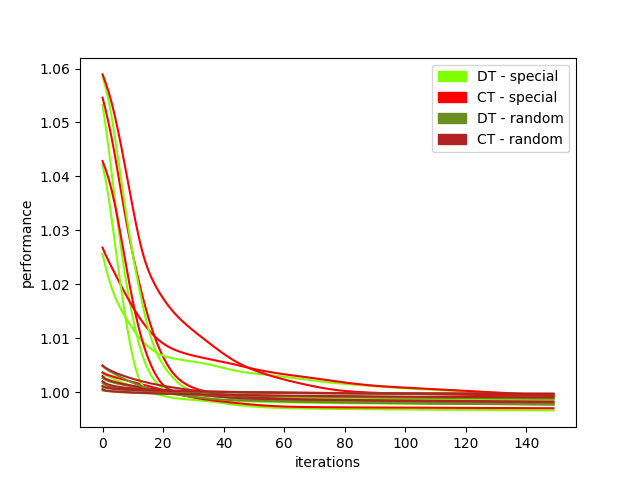
\includegraphics[width=1\linewidth]{img/ex1/2/all.png}
  \captionof{figure}{Average convergences for various generated datasets.}
  \label{fig:all}
\end{minipage}
\begin{minipage}{.8\textwidth}
  \centering
  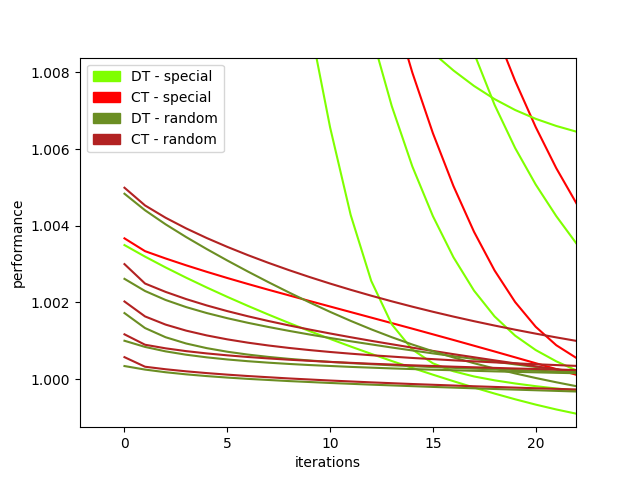
\includegraphics[width=.95\linewidth]{img/ex1/2/random.png}
  \captionof{figure}{Average convergences for various generated datasets (zoom).}
  \label{fig:random}
\end{minipage}
\end{figure}  

\subsection{ Conclusions }

The slower convergence of continuous-time model is bounded with the different character of the model. Since in the discrete-time model we always know, the precise time, when the state-change can happen (always at observation point), in continuous-time model it can happen in any time in between as well. Thus, the computing of the new estimated parameters in maximization step needs to deal with more unknown. 
In continuous-time model is uncertainty not only caused by indirect observation of hidden states, but also by possible state changes in between of the observations. As we have any observations from that area, the probability estimation will be counted by parameters from the last iteration, what is creating the momentum in favor of old parameters and slow down the convergence process. The longer is the time interval, the stronger is the momentum.

In the second experiment we have showed, how the characteristic of the searched model influenced the training complexity. The randomly generated models usually generate datasets with higher entropy. Such datasets are closer to converge from most regions of the parameter space. 

The over-performing of the original model is caused by the over-fitting. the small size of dataset was not sufficient to cover characteristic of the model completely, instead the trained models were learned to fit its imprecision. It is not a problem for our experiment as the original models were chosen more-less randomly and it fill in its purpose. The over-performing would probably gradually disappear with growing size of the data-set. It will be shown in experiment \ref{sec:plast}.

%TODO All of the training conducted during this experiment, more or less converged to something, what seems to be global optima. We have used the simple 3-states models, the behavior of more complex models will be examined later in [odkaz].    
 	


\section{Computational Complexity}\label{sec:cc}

In this section we are comparing time-performance of the float and integer-interval variants of CT-HMM  as described in implementation part \ref{sec:alg}.
In two following subsection we experimented either with  variable hidden states number or maximal time interval and examined, if the measured values correspond to their theoretical expectations described in section \ref{sec:complex}.

\subsection{Variable Hidden-states Number}

The hidden states number, referred to as $n$ is the key parameter in overall algorithm complexity. Due to computing of the matrix exponentials ($n^3$) for every pair of end states, it influence the final time-complexity by its fifth power $n^5$. The upper bound theoretical complexity dependence on $n$ is the same for both of the variants. However, the float-algorithm counts the matrix exponential by \textit{expm} method separately for every time interval, while the integer-algorithm counts it only once and then use the matrix multiplication to get the individual results \ref{it:ctc}. In the experiment we measure and compare the times of most costly algorithm parts, and notice how big is the portion of the overall computational complexity consumed by them. 

\begin{itemize}
\item \textbf{ Description }

[ the itemize looks weird, but is it more weird than subsubsection ? ] %TODO

We have trained the models with the variable number of hidden states. To minimize the impact of the other factors, we have let the number of output variables to be constantly 10 and we have used the same randomly generated dataset for both algorithm variants. The integral times intervals were generated by exponential distribution with parameter 0.5. To minimize the time measurements error, we have always run 10 iterations of algorithm and repeated the all procedure 5 times. 

To see how the size of the dataset influence time-demand, we have conducted all the described experiment twice. Once with the \textit{small} dataset - compounding 10 sequences of 10 observations and once with the \textit{big} dataset - compounding 10 sequences of 100 observations.  

\item \textbf{ Observation }

On the figure \ref{fig:e2n}, we can observe that the float-interval algorithm is always slower. The prevalent source of complexity is the \textit{expm} method. In the float-interval algorithm over the small dataset are all other parts of the algorithm almost neglectable comparing to it.

Comparing to the \textit{expm} are the time-demands of \textit{square and multiply} algorithm considerably smaller. It is called multiple times over different time-intervals and still takes smaller portion of the time as the single \textit{expm} call.

The increase of the dataset size caused the larger gap among the whole algorithm time-complexity and its measured subparts - either \textit{expm} or the sum of \textit{expm} and \textit{square and multiply} depending on the algorithm \ref{fig:e2big}.   

\begin{figure}
\centering
\begin{subfigure}{.8\textwidth}
  \centering
  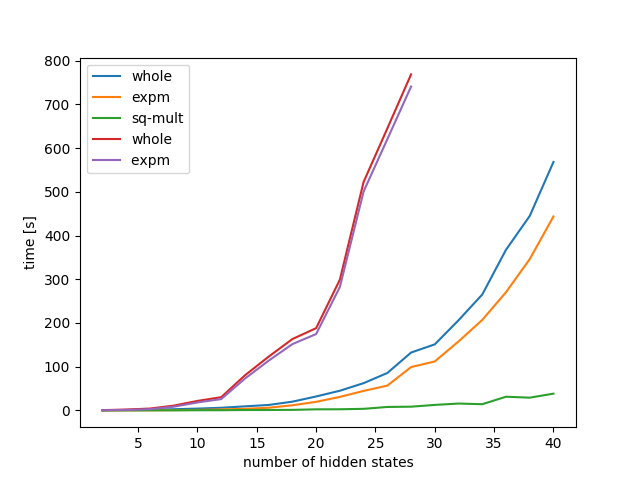
\includegraphics[width=1\linewidth]{img/ex2/small.png}
  \caption{Small dataset}
  \label{fig:e2small}
\end{subfigure}
\begin{subfigure}{.8\textwidth}
  \centering
  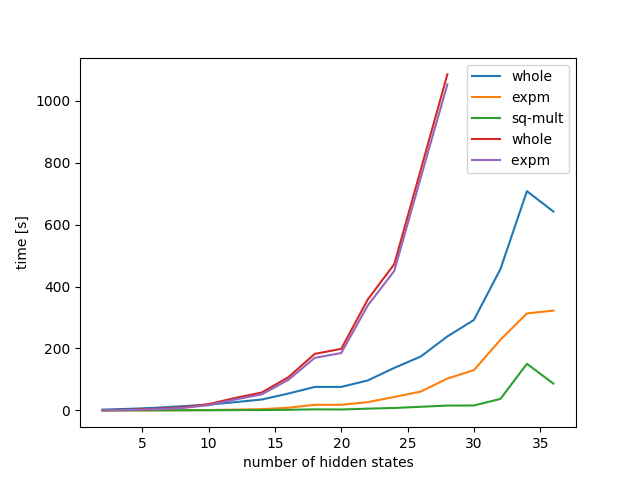
\includegraphics[width=\linewidth]{img/ex2/big.png}
  \caption{Big dataset}
  \label{fig:e2big}
\end{subfigure}
\caption{ The time-complexity of the two algorithm variants and their subparts }
\label{fig:e2n}
\end{figure}

\item \textbf{ Conclusion }

We have only changed the number of states and let the dataset to be the same, so the $t_{\max}$ parameter from the integer-interval complexity $\mathcal{O}(r n^5 \log(t_{\max}))$ is fixed as constant. This makes both both algorithm variants to have same complexity $\mathcal{O}(r*n^5)$. The measurements have shown, the big multiplicative constant of \textit{expm} method. That's way it is almost always better, if possible to use the integer-interval algorithm. (Its numerical stability is tested later in section \ref{sec:ns}) 

The most of the computational power is used to count matrix exponentials $expm$. In most cases it is the predominant cause of algorithm "slowness". It makes not much sense to edge-optimize other parts of the algorithm. Instead, the faster implementation of \textit{expm}, its parallelization or replacement with other method could spare the significant portion of time.      

Training over the big dataset \label{fig:e2big} has decreased the percentage of the time spent by $expm$ method. It is because the higher demand of other algorithm parts. Potentially, it can happen that this gap would overgrowth the $expm$ part. The complexity of the algorithm part that call $expm$ method only depend on $r$ - the number of different time intervals, however there are parts of the algorithms with complexity ${O}(n^2T)$ \ref{it:ctc}, where $T$ is number of all time intervals. So for the huge dataset with lower number of hidden states and many identical time intervals can this part be the predominant cause of the complexity.   

\end{itemize}

\subsection{Variable Maximal Time Interval}

The other parameter presented in the theoretical time-complexity of the integer-interval algorithm - $\mathcal{O}(r n^5 \log(t_{\max}))$ is $t_{\max}$ - maximal length of the time interval. On the oder side the parameter is not part of the float-interval algorithm complexity term - $\mathcal{O}(r n^5)$ \ref{it:ctc}. The experiment aims to observe how the variable value of $t_{\max}$ change the computational demand of the algorithm.  

\begin{itemize}
\item \textbf{ Description }

In the experiment we have set $t_{\max}$ as the variable, taking values of powers of two from $2^1$ to $2^{56}$. The use of higher values (even floats) was impossible, because of conversion to 64-bites integer used in \textit{SciPy} \textit{expm} method, that eventually causes the integer overflow. We have generated the dataset of 10 sequences by 10 observations. There was always at least one time-interval of length $t_{\max}$ and all other were chosen uniformly from interval $[1,t_{\max}]$. We have trained the model of $10$ hidden states and $10$ observation variables. To smooth the influence of the time measurement imprecision, we have run $10$ iterations and repeated the whole experiment $5$ times.   

\item \textbf{ Observation }

Contrary to initial expectation both float and integer interval algorithm computational times are growing seemingly logarithmically with increasing $t_{\max}$. The cause of growth in float-interval algorithm is \textit{expm} method, in integer-interval algorithm it is caused mainly by \textit{square and multiply} method. There is the steep growth of the float-interval algorithm time demand present for small $t_{\max}$ values.

\begin{figure}[h]
\centering
\begin{minipage}{.8\textwidth}
  \centering
  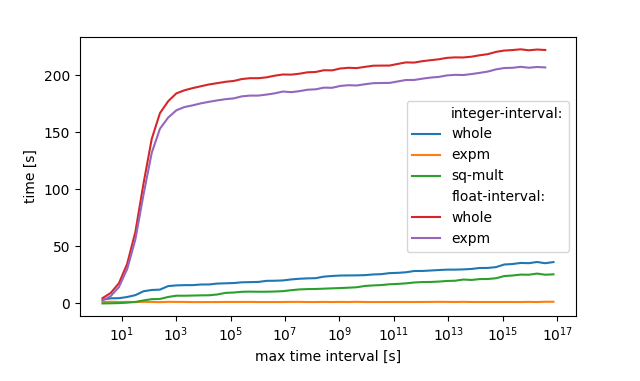
\includegraphics[width=1.0\linewidth]{img/ex2/log.png}
  \captionof{figure}{log.}
  \label{fig:e2log}
\end{minipage}
\begin{minipage}{.8\textwidth}
  \centering
  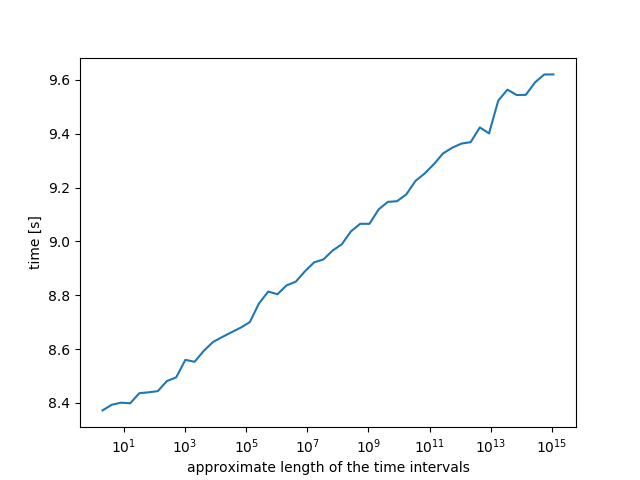
\includegraphics[width=1.0\linewidth]{img/ex2/exp180.png}
  \captionof{figure}{log2.}
  \label{fig:e2big}
\end{minipage}
\end{figure}

\item \textbf{ Conclusion }

The steep growth at the beginning is caused by choice of integral interval lengths. For small values of $t_{\max}$ is higher probability of more same-sized time-intervals. That has direct impact at the complexity, where variable $r$ is directly present. The chance of choosing two same interval length for bigger $t_{\max}$ values is extremely low.

The logarithmic grow of \textit{square and multiply} method is obvious. But to explain similar behavior of the $expm$ method, we need to look deeper in its implementation \cite{Sc01}. %[https://github.com/scipy/scipy/blob/v0.16.1/scipy/sparse/linalg/matfuncs.py#L554]. 
The method is using Pad\'{e} approximants of different values from $3$ to $13$. The computation of the approximants of higher order is computationally more costly. The algorithm is choosing the smallest  Pad\'{e} approximant, which securely not overgrow the wished threshold error. Our observation suggest, that the bigger the numbers in the exponentiated matrix are, the bigger is the probability that the more complex Pad\'{e} approximant will be chosen.   %TODO odkaz na clanok co to robi?-zo scipy  

\end{itemize}

\begin{itemize} %TODO vymaz alebo pridaj posledny experiment s pade.
\item \textbf{ Description }
\item \textbf{ Observation }
\item \textbf{ Conclusion }
\end{itemize}


\section{Numerical Stability}\label{sec:ns} 

The main advantage of integer-interval variant of algorithm is that it computes the costly matrix exponential only once and derive all other exponentials of the matrix multiplications by computing its powers, via \textit{square and multiply} method. It arise the question of numerical stability of the method. Can the inaccuracies acquired by \textit{square and multiply} significantly change the direction of convergence?   

\begin{itemize}
\item \textbf{ Description }
In the experiment we have run both integer and float-algorithms with the same initial parameters. As the value of interest, we have measured the relative euclidean distance among both models jump-rates matrices $\matr{Q}$. We have used the models of $5$ hidden states and $5$ observable variables at the dataset of $100$ observation points. The time intervals were generated by exponential distribution with parameter $\lambda$ equal $0.1$, $0.01$ and $0.001$ consecutively. The obtained plotted error is the average value of $10$ runs of the experiment.      

\item \textbf{ Observation }

The measured relative distance of jump-rate matrices seems to be random and it doesn't significantly increase by the growing iteration number. However it seems that the variance magnitude grows with the decreasing magnitude of exponential parameter $\lambda$.   


\begin{figure}
\centering
\begin{subfigure}{.7\textwidth}
  \centering
  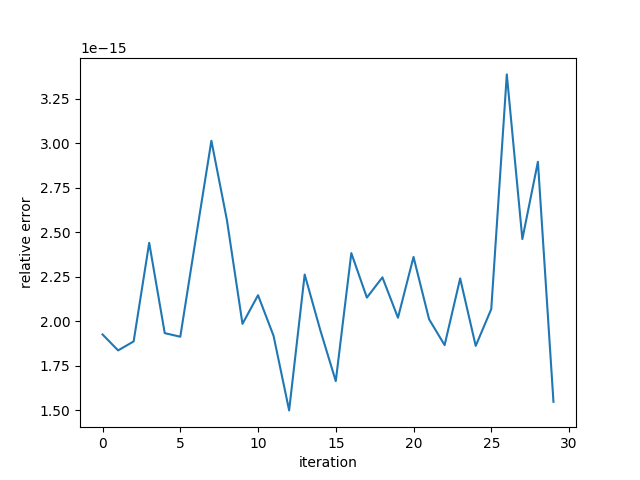
\includegraphics[width=1\linewidth]{img/ex3/relative01.png}
  \caption{ $\lambda = 0.1$ }
  \label{fig:sub1}
\end{subfigure}
\begin{subfigure}{.7\textwidth}
  \centering
  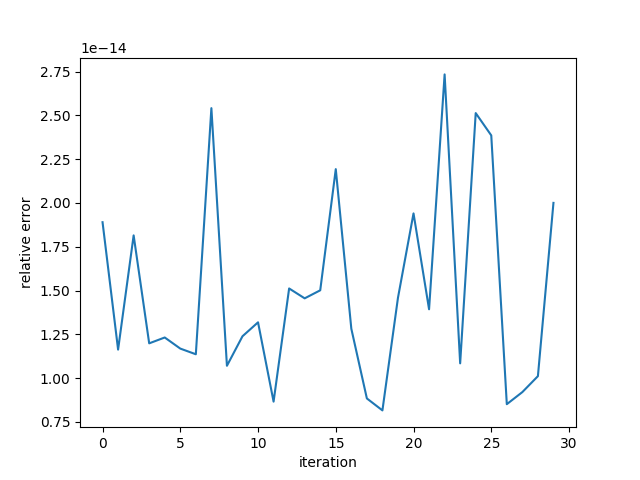
\includegraphics[width=1\linewidth]{img/ex3/relative001.png}
  \caption{$\lambda = 0.01$}
  \label{fig:sub1}
\end{subfigure}
\begin{subfigure}{.7\textwidth}
  \centering
  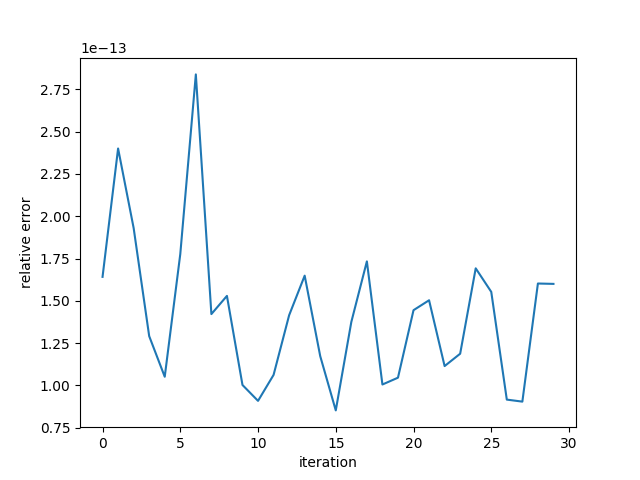
\includegraphics[width=1\linewidth]{img/ex3/relative0001.png}
  \caption{$\lambda = 0.001$}
  \label{fig:sub2}
\end{subfigure}
\caption{Relative distances of jump-rates matrices for data generated with different exponential distribution parameter $\lambda$}
\label{fig:test}
\end{figure}

\item \textbf{ Conclusion }
The experiment haven't shown any error propagation by growing the iterations number. So the errors seems to be eliminated as they decrease to the local optima. It is not the proof and it is probable, that under some more extreme edge conditions the matrices may diverge. But, when taking into the account the randomness of the initial configuration and assorted characteristic of the parameter space, we do not see it as problem and we do not think it can, in general, negatively influence the performance of the algorithm.  

\end{itemize}

\section{Soft-Hard}

\begin{itemize}
\item \textbf{ Description }
\item \textbf{ Observation }

\begin{figure}
\centering
\begin{subfigure}{.8\textwidth}
  \centering
  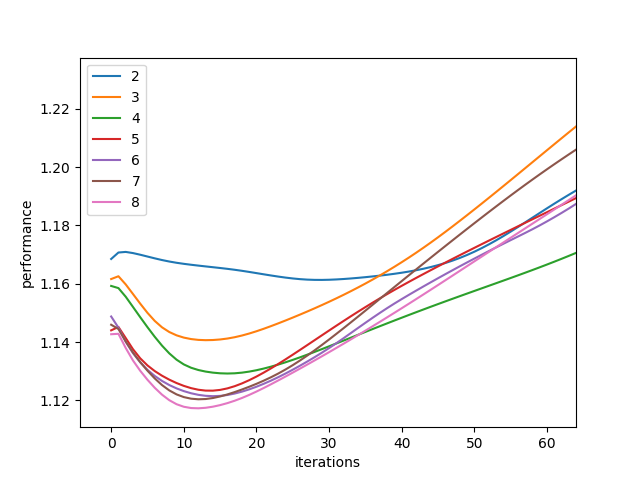
\includegraphics[width=1\linewidth]{img/ex5/test_small.png}
  \caption{A subfigure}
  \label{fig:sub1}
\end{subfigure}
\begin{subfigure}{.8\textwidth}
  \centering
  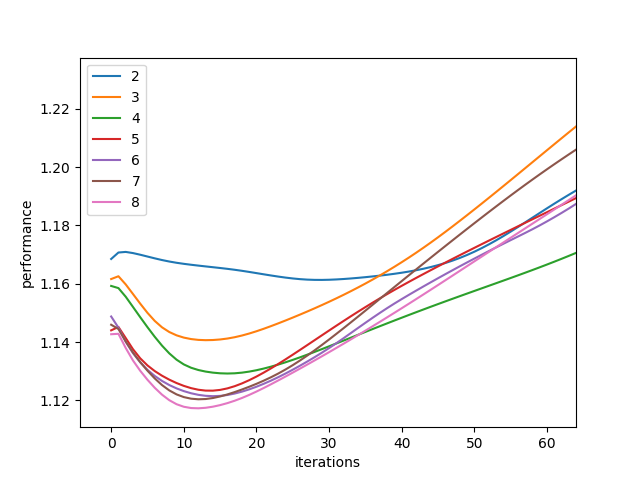
\includegraphics[width=1\linewidth]{img/ex5/test_small.png}
  \caption{A subfigure}
  \label{fig:sub2}
\end{subfigure}
\caption{A figure with two subfigures}
\label{fig:test}
\end{figure}

\begin{figure}
\centering
\begin{subfigure}{.8\textwidth}
  \centering
  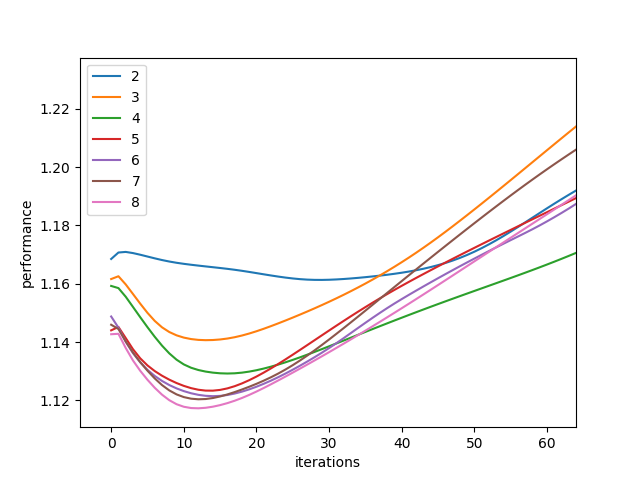
\includegraphics[width=1\linewidth]{img/ex5/test_small.png}
  \caption{A subfigure}
  \label{fig:sub1}
\end{subfigure}
\begin{subfigure}{.8\textwidth}
  \centering
  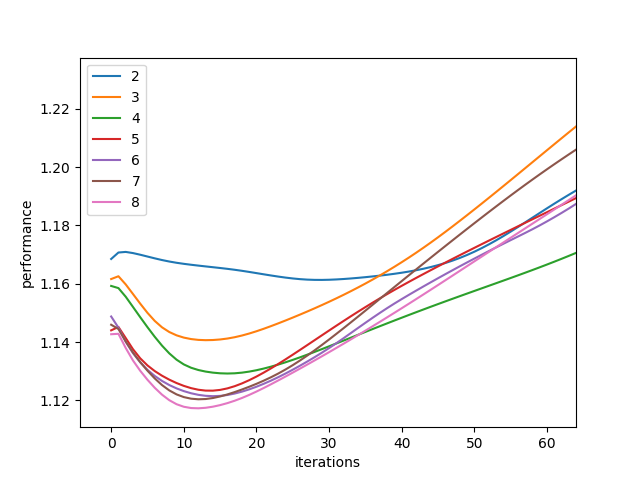
\includegraphics[width=1\linewidth]{img/ex5/test_small.png}
  \caption{A subfigure}
  \label{fig:sub2}
\end{subfigure}
\caption{A figure with two subfigures}
\label{fig:test}
\end{figure}

\item \textbf{ Conclusion }
\end{itemize}


\section{Hidden States Number}\label{sec:hsn}

The number of hidden states is an important parameter, influencing the characteristic of the model. The higher number means the higher plasticity of the model. It can be beneficial as the model can better fit the domain space, however sometimes it may not be useful at all and cause the over-training. The parameter also critically influence the time and memory complexity of the algorithm. In following two experiments we will observe, how variable number of states behave, when matching the dataset generating by single model, and in the later we will try to find the limits of the algorithm regarding the number of states and examine how the increasing complexity of the parameter space influence the convergence ability.    

\subsection{Plasticity of the Models}\label{sec:plast}

\begin{itemize}
\item \textbf{ Description }
For this experiment we have created an artificial model consisting of five hidden states arranged in the way of birth and death chain as in the figure \ref{??}. There is not allowed for the model to change states except in the way of arrows. However to add the uncertainty into the dataset, we have blurred the observation symbol emission by adding the $15\%$ error to the emitted symbol. The model is deliberately build in the way, so it uncovers the properties worthy to explore. However the properties are more or less visibly present in any model. 

%TODO
%\begin{figure}
%\centering
%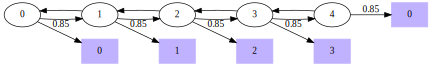
\includegraphics[width=1\linewidth]{img/ex5/hs.svg}
%caption{...}
%\label{fig:bg}
%\end{figure}
 
We have generated three random datasets. The \textit{small} training dataset consisting of $15$ sequences each by $15$ observations and two \textit{big} datasets of $100$ sequences by $100$ observations, one for training and other for testing purpose. We have used both training datasets to train models with variable number of hidden states (from 2 to 8) and marked their performance after every of one hundred iteration at the respective training and \textit{big} testing dataset. We have repeated the experiments five times and plotted the average results.   

\item \textbf{ Observation }

The models, except the ones with 2 and 3 hidden states, were able to over-perform the original model at the \textit{small} training dataset after couple of iterations\ref{fig:smtrain}. The bigger number of hidden states makes the convergence faster and also converge to the lower value. The measure at the testing dataset shows, that the models were actually over-fitted after couple of iterations and later diverge from the actual model. \ref{fig:smtest}. 

On the contrary the convergence lines plotting the training on the \textit{big} dataset \ref{fig:bgtrain} are almost the same as results on the testing data \ref{fig:bgtest}. Models with the hidden states number higher or equal 5 converge well. After one hundred iteration they have reached performances in interval $[1.00025,1.006]$ on the training dataset and $[1.0032-1.01]$ on the testing dataset. Higher number of states make the convergence faster, but all of the models seems to converge to the similar value. Models with the 4 or lower number of hidden states converge visibly worse. 

\begin{figure}
\centering
\begin{subfigure}{.8\textwidth}
  \centering
  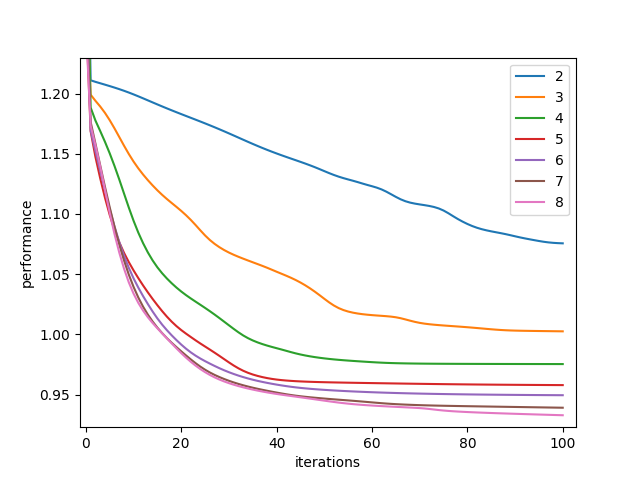
\includegraphics[width=1\linewidth]{img/ex5/train_small.png}
  \caption{Performance on the \textit{small} training dataset}
  \label{fig:smtrain}
\end{subfigure}
\begin{subfigure}{.8\textwidth}
  \centering
  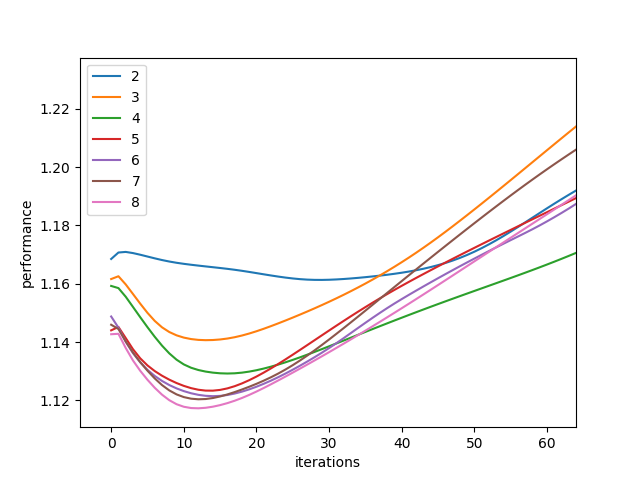
\includegraphics[width=1\linewidth]{img/ex5/test_small.png}
  \caption{Performance on the testing dataset}
  \label{fig:smtest}
\end{subfigure}
\caption{Performance of the models with variable hidden states number trained by the \textit{small} dataset}
\label{fig:sm}
\end{figure}

\begin{figure}
\centering
\begin{subfigure}{.8\textwidth}
  \centering
  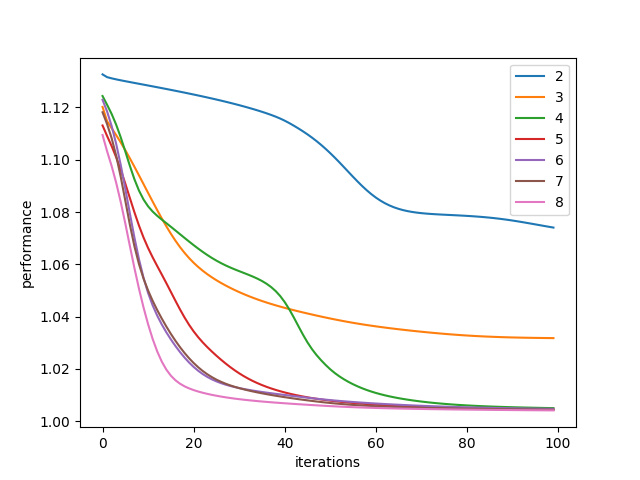
\includegraphics[width=1\linewidth]{img/ex5/train_big.png}
  \caption{Performance on the \textit{big} training dataset}
  \label{fig:bgtrain}
\end{subfigure}
\begin{subfigure}{.8\textwidth}
  \centering
  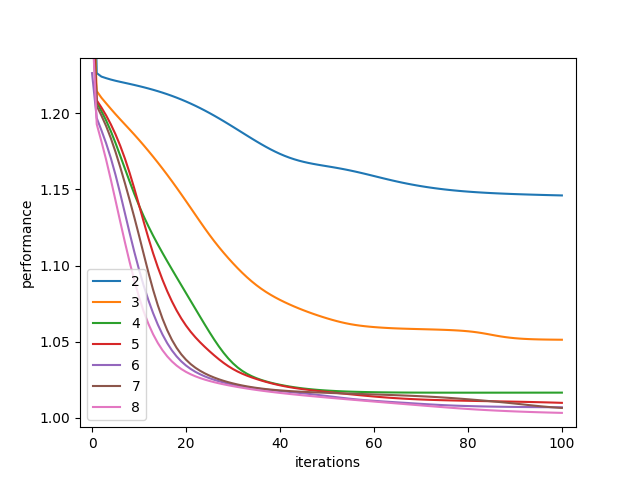
\includegraphics[width=1\linewidth]{img/ex5/test_big.png}
  \caption{Performance on the testing dataset}
  \label{fig:bgtest}
\end{subfigure}
\caption{Performance of the models with variable hidden states number trained by the \textit{big} dataset}
\label{fig:bg}
\end{figure}

\item \textbf{ Conclusion }
Choosing the correct number of hidden states is crucial as its under-valuating can negatively influence the performance of the algorithm. Insufficient number of the hidden states for models 2-4 does not allow them to converge to the optimum values. The waves on the convergence lines of models 2 and 3 reveal that the averaged convergence lines differ. That marks the instability, thus the model that is too weak to cover the problem space. Model 4 was probably not able to distinguish the states at the ends of the birth and death sequence, that's way it has not reached the peak performance.

We haven't proof that the over-valuated number of hidden states makes the models more vulnerable to over-fitting, as all models has over-fitted similarly. The higher number of states than in the original model makes the model to converge in the smaller number of iterations, but not to the considerably better values. However, the cost of computationally more expensive single iteration makes their convergence slower in real time.

The experiment also stresses the importance of sufficiently sized dataset, as the small one emphasized the statistical error and lead to the over-fitting of the models. That is not the surprise, the weak dataset can't train powerful model. 
\end{itemize}


% expm reference form scipy: The Scaling and Squaring Method for the Matrix Exponential Revisited",
%    SIAM. J. Matrix Anal. & Appl. 26, 1179 (2005).

%http://mathoverflow.net/questions/239073/what-is-the-time-complexity-of-the-matrix-exponential/239083


%\chapter{Realisation}

\setsecnumdepth{part}
\chapter{Conclusion}

malo informacie (vela hidden) menej presny.
rychlo sa straca informacia 

\section{Future Work}


\bibliographystyle{iso690}
\bibliography{bibliography}

\setsecnumdepth{all}
\appendix

\chapter{Acronyms}
% \printglossaries
\begin{description}
	\item[DTMP] Discrete-time Markov Process	
	\item[CTMP] Continuous-time Markov Process
	\item[DT-HMM] Discrete-time Hidden Markov Model
	\item[CT-HMM] Continuous-time Hidden Markov Model
	\item[EM] Expectation-Maximization 
	\item[MLE] Maximum likelihood estimation
\end{description}


\chapter{Contents of enclosed CD}

%change appropriately

\begin{figure}
	\dirtree{%
		.1 readme.txt\DTcomment{the file with CD contents description}.
		.1 exe\DTcomment{the directory with executables}.
		.1 src\DTcomment{the directory of source codes}.
		.2 wbdcm\DTcomment{implementation sources}.
		.2 thesis\DTcomment{the directory of \LaTeX{} source codes of the thesis}.
		.1 text\DTcomment{the thesis text directory}.
		.2 thesis.pdf\DTcomment{the thesis text in PDF format}.
		.2 thesis.ps\DTcomment{the thesis text in PS format}.
	}
\end{figure}

\end{document}
